\documentclass{beamer}

\mode<presentation> {
	\usetheme{Antibes}
	\setbeamertemplate{footline}[page number]	
	\setbeamertemplate{navigation symbols}{}
	\setbeamertemplate{items}[square]
}

\usepackage{graphicx}
\usepackage{booktabs}
\usepackage{hyperref}

\newcommand{\link}[2]{\href{#1}{\textit{\color{blue}{#2}}}}%


\title[DragonFly]{Project DragonFly: Vehicle Surveillance System}
\institute[GCEK-CSE]{Department of Computer Science and Engineering \\Government College of Engineering Kannur}
\author[Group 3]{
	{\small \textit{Guided by:}} Dr. Rafeeque P.C \\
	\medskip
	{\small \textbf{\textit{Group 3}}} \\
	Abhinand C \\ Edwin Jose George \\ Lavanya E.V \\ Shilpa Suresh
}
\date{\today}

%Conclusion
%Future Scope
% challange and future emprovemtns
%References


\begin{document}
	
	%---------------------------------------------------------------------------
	% METADATA -----------------------------------------------------------------
	%---------------------------------------------------------------------------

	\begin{frame}
	\titlepage
	\end{frame}

	\begin{frame}{Table of Contents}
	\tableofcontents
	\end{frame}


	%---------------------------------------------------------------------------
	% INTRODUCTION -------------------------------------------------------------
	%---------------------------------------------------------------------------

	\section{Introduction}
	\subsection{Motivation}
	\begin{frame}{Motivation}
		\begin{itemize}
			\item Policing agencies have setup vast networks of distributed surveillance cameras along major routes. The sheer amount of data generated is overwhelming for manual analysis, to trace routes of rouge vehicles.
			\item Current system make use of manual approach of reviewing long video
			clips to identify the suspect vehicle. Various possible routes that can
			be taken by suspect further makes the process of re-identification very
			difficult and time consuming.		
		\end{itemize}
		
		\begin{block}{Open AI city challenge}
			This is one of the open challenges in NVIDIA AI city challenge, to perform Natural language-based vehicle track retrieval and City-scale multi-camera vehicle tracking.
		\end{block}
		
	\end{frame}

	\subsection{Objective}
	\begin{frame}{Objective}
		\begin{itemize}
			\item Aid in traffic policing by extracting and detecting various vehicle
			description from existing CCTV infrastructure
			\item Generate route map for a specific vehicle description, along with timestamps, visualized in minimalist user interface. 
			\item Conduct traffic analysis to predict traffic flow with existing sensor
			network, and generate probabilistic patterns for resource deployment.
			\item Easier management \& visualization of CCTV camera infrastructure
		\end{itemize}
	\end{frame}

	\subsection{Literature Review}
	\begin{frame}{Literature Review}
		\begin{table}[!h]
			\centering
			\resizebox{\textwidth}{!}{%
				\begin{tabular}{|l|l|l|l|}
					\hline
					\multicolumn{1}{|c|}{\textit{\textbf{Title}}} &
					\multicolumn{1}{c|}{\textit{\textbf{Method}}} &
					\multicolumn{1}{c|}{\textit{\textbf{Pros and Cons}}} &
					\multicolumn{1}{c|}{\textit{\textbf{Challenges}}} \\ \hline
					\begin{tabular}[c]{@{}l@{}}CityFlow: A City-Scale \\ Benchmark for Multi-Target\\ Multi-Camera  Vehicle\\  Tracking and  \\ Re-Identification, 2019\end{tabular} &
					\begin{tabular}[c]{@{}l@{}}Use of Multi-Target Single Camera\\ and Multi-Target Multi-Camera \\ tracking.\\ \\ Use visual-spatio-temporal\\ reasoning\end{tabular} &
					\begin{tabular}[c]{@{}l@{}}Pros:\\ Better and faster results.,\\ Handle large scale recognition\\ Tracking and small prediction\\ \\ Cons:\\ Overlapping viewpoints,\\ Implemented only at junction \\ points\end{tabular} &
					\begin{tabular}[c]{@{}l@{}}High quality videos\\ \\ Multiple viewpoints on \\ same object\\ \\ Require annotated videos\end{tabular} \\ \hline
					\begin{tabular}[c]{@{}l@{}}Real-Time Vehicle Make and\\ Model Recognition System, 2019\end{tabular} &
					\begin{tabular}[c]{@{}l@{}}Random Forest and Support Vector\\  Machine coupled with traditional\\ Vehicle Make Model Recognition\\ System,\\ \\ Usage of Histogram of Oriented \\ Gradient (HOG) and GIST \\ features\end{tabular} &
					\begin{tabular}[c]{@{}l@{}}Pros:\\ Superior processing speed \& \\ recognition accuracy wrt existing \\ VMMR, Accounts for partial \\ viewpoints\\ \\ Cons:\\ High dimensional,  Region of \\ interest is only on parts, No global\\  representation\end{tabular} &
					\begin{tabular}[c]{@{}l@{}}Computational time increases\\ with increase of blocks HOG\\ \\ Limited Region of Interest\end{tabular} \\ \hline
					\begin{tabular}[c]{@{}l@{}}Efficient and Deep Vehicle \\ Re-Identification Using \\ Multi-Level Feature \\ Extraction, 2019\end{tabular} &
					\begin{tabular}[c]{@{}l@{}}Global channel extracts single \\ feature generalizing whole image,\\ \\ Local channel extract multiple\\  local features (logo, stickers),\\ \\ Attribute channel extracts \\ color, model, type\end{tabular} &
					\begin{tabular}[c]{@{}l@{}}Pros:\\ Extraction of inter and intra features,\\ Data augmentation with license plate \\ verification\\ \\ Cons:\\ Requires Data augmentation,\\ Effected by illuminations\end{tabular} &
					\begin{tabular}[c]{@{}l@{}}Cross camera vehicle tracking\\ \\ Changes in color response\\ \\ Background clutter\end{tabular} \\ \hline
				\end{tabular}%
			}
		\end{table}
		% include NVIDIA AI challange, papers regarding yolov4, paddlepaddle, github repository
	\end{frame}

	\subsection{Problem Statement}
	\begin{frame}{Problem Statement}
		A novel approach to provide an integrated platform utilizing existing infrastructure to monitor transport sector, and extend timely information to policing agencies, with intuitive interface.
	\end{frame}

	\begin{frame}{Contributions}
		\begin{itemize}
			\item Custom YOLOv4 AI model trained on Indian vehicles
			\item Integration of various AI based algorithm and models (YOLOv4, deepSORT, siamese Network)
   			\item Vehicle Image Dictionary Framework - to enable easier identification and labeling 
			\item Minimalistic user interface
			\item Wiregaurd VPN based interface for securely connecting with existing CCTV infrastructure
   			\item Websocket based interactive realtime tracking UI 
			\item Containerised CI/CD pipeline 
			\item Secure HLS based Camera Live Streaming
		\end{itemize}
	\end{frame}

	\begin{frame}{Challenges Faced}
		\begin{itemize}
			\item SOCKS5 Proxy not working on system level and OpenCV not able to stream
			\item RTMP not supporting HEVC, Nginx requires RTMP ingress, IP camera give RSTP HEVC 
   			\item Google Colab not allowing training for long duration
			\item Accessing system inside and outside NAT
			\item Online Dataset \& Nvidia Dataset acquired not reflecting indian roads
   			\item Tedious and time consuming process of Dataset labelling, identification of class 
		\end{itemize}
	\end{frame}
	
	
	%---------------------------------------------------------------------------
	% DESIGN AND IMPLEMENTATION ------------------------------------------------
	%---------------------------------------------------------------------------	
	
	\section{Design and Implementation}
	\begin{frame}{Proposed System}
		\begin{itemize}
			\item The user provides the system with vehicle descriptions such as color, model, location, time-period etc. 
			\item The system finds corresponding match by making use of various AI techniques. 
			\item The system tries to re-identify the said vehicle across multiple camera locations.
			\item The system finds the path followed by the said vehicle along with the detected frame at each camera points.
		\end{itemize}
	\end{frame}

	\begin{frame}{IP Camera Infrastructure}
		\framesubtitle{CICET Camera Network}
		\begin{center}
			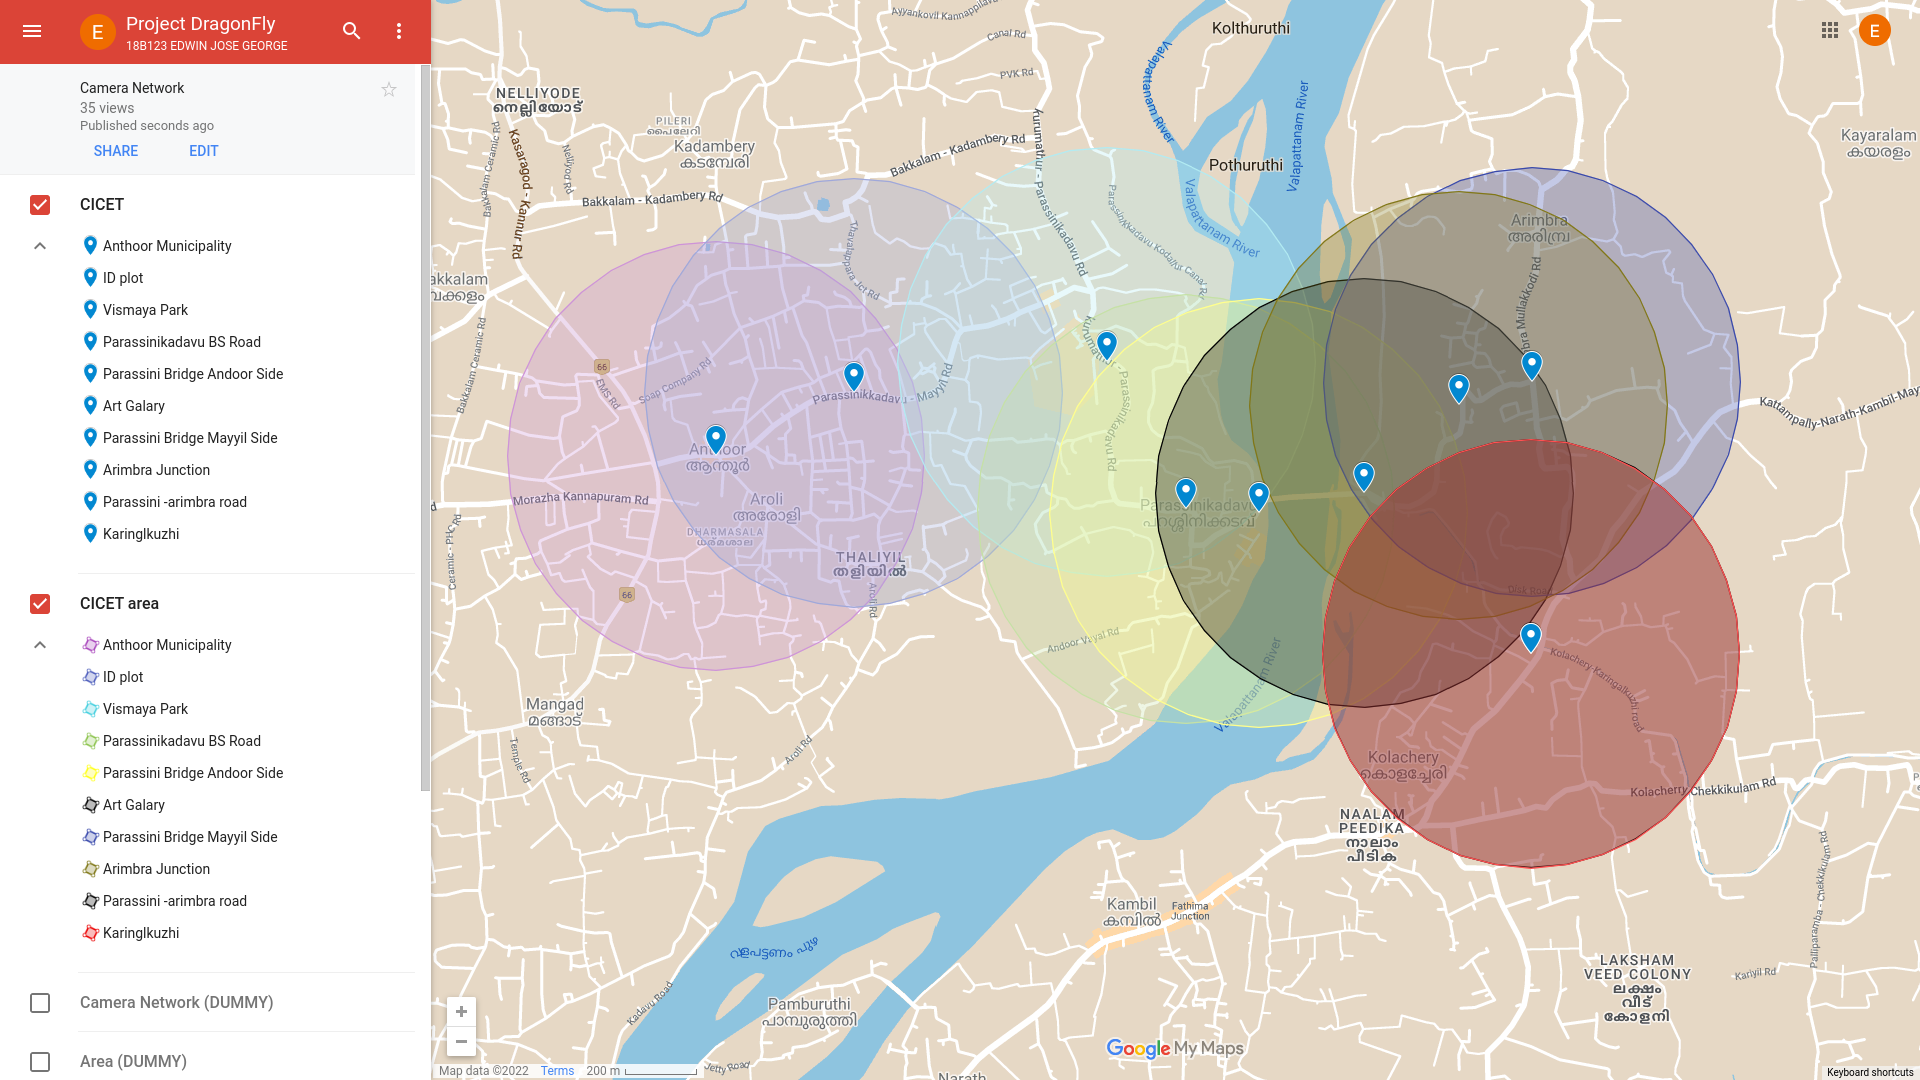
\includegraphics[height=0.7\textheight]{res/camera-network.png}
		\end{center}
		Created with \link{https://www.google.com/maps/d/edit?mid=1s2ST5x4nn-EK3JqU-c9EEGASRq5Ini0&usp=sharing}{Google Maps}
	\end{frame}
	
	\subsection{System Architecture}
	\begin{frame}{Architecture Design}
		\begin{center}
			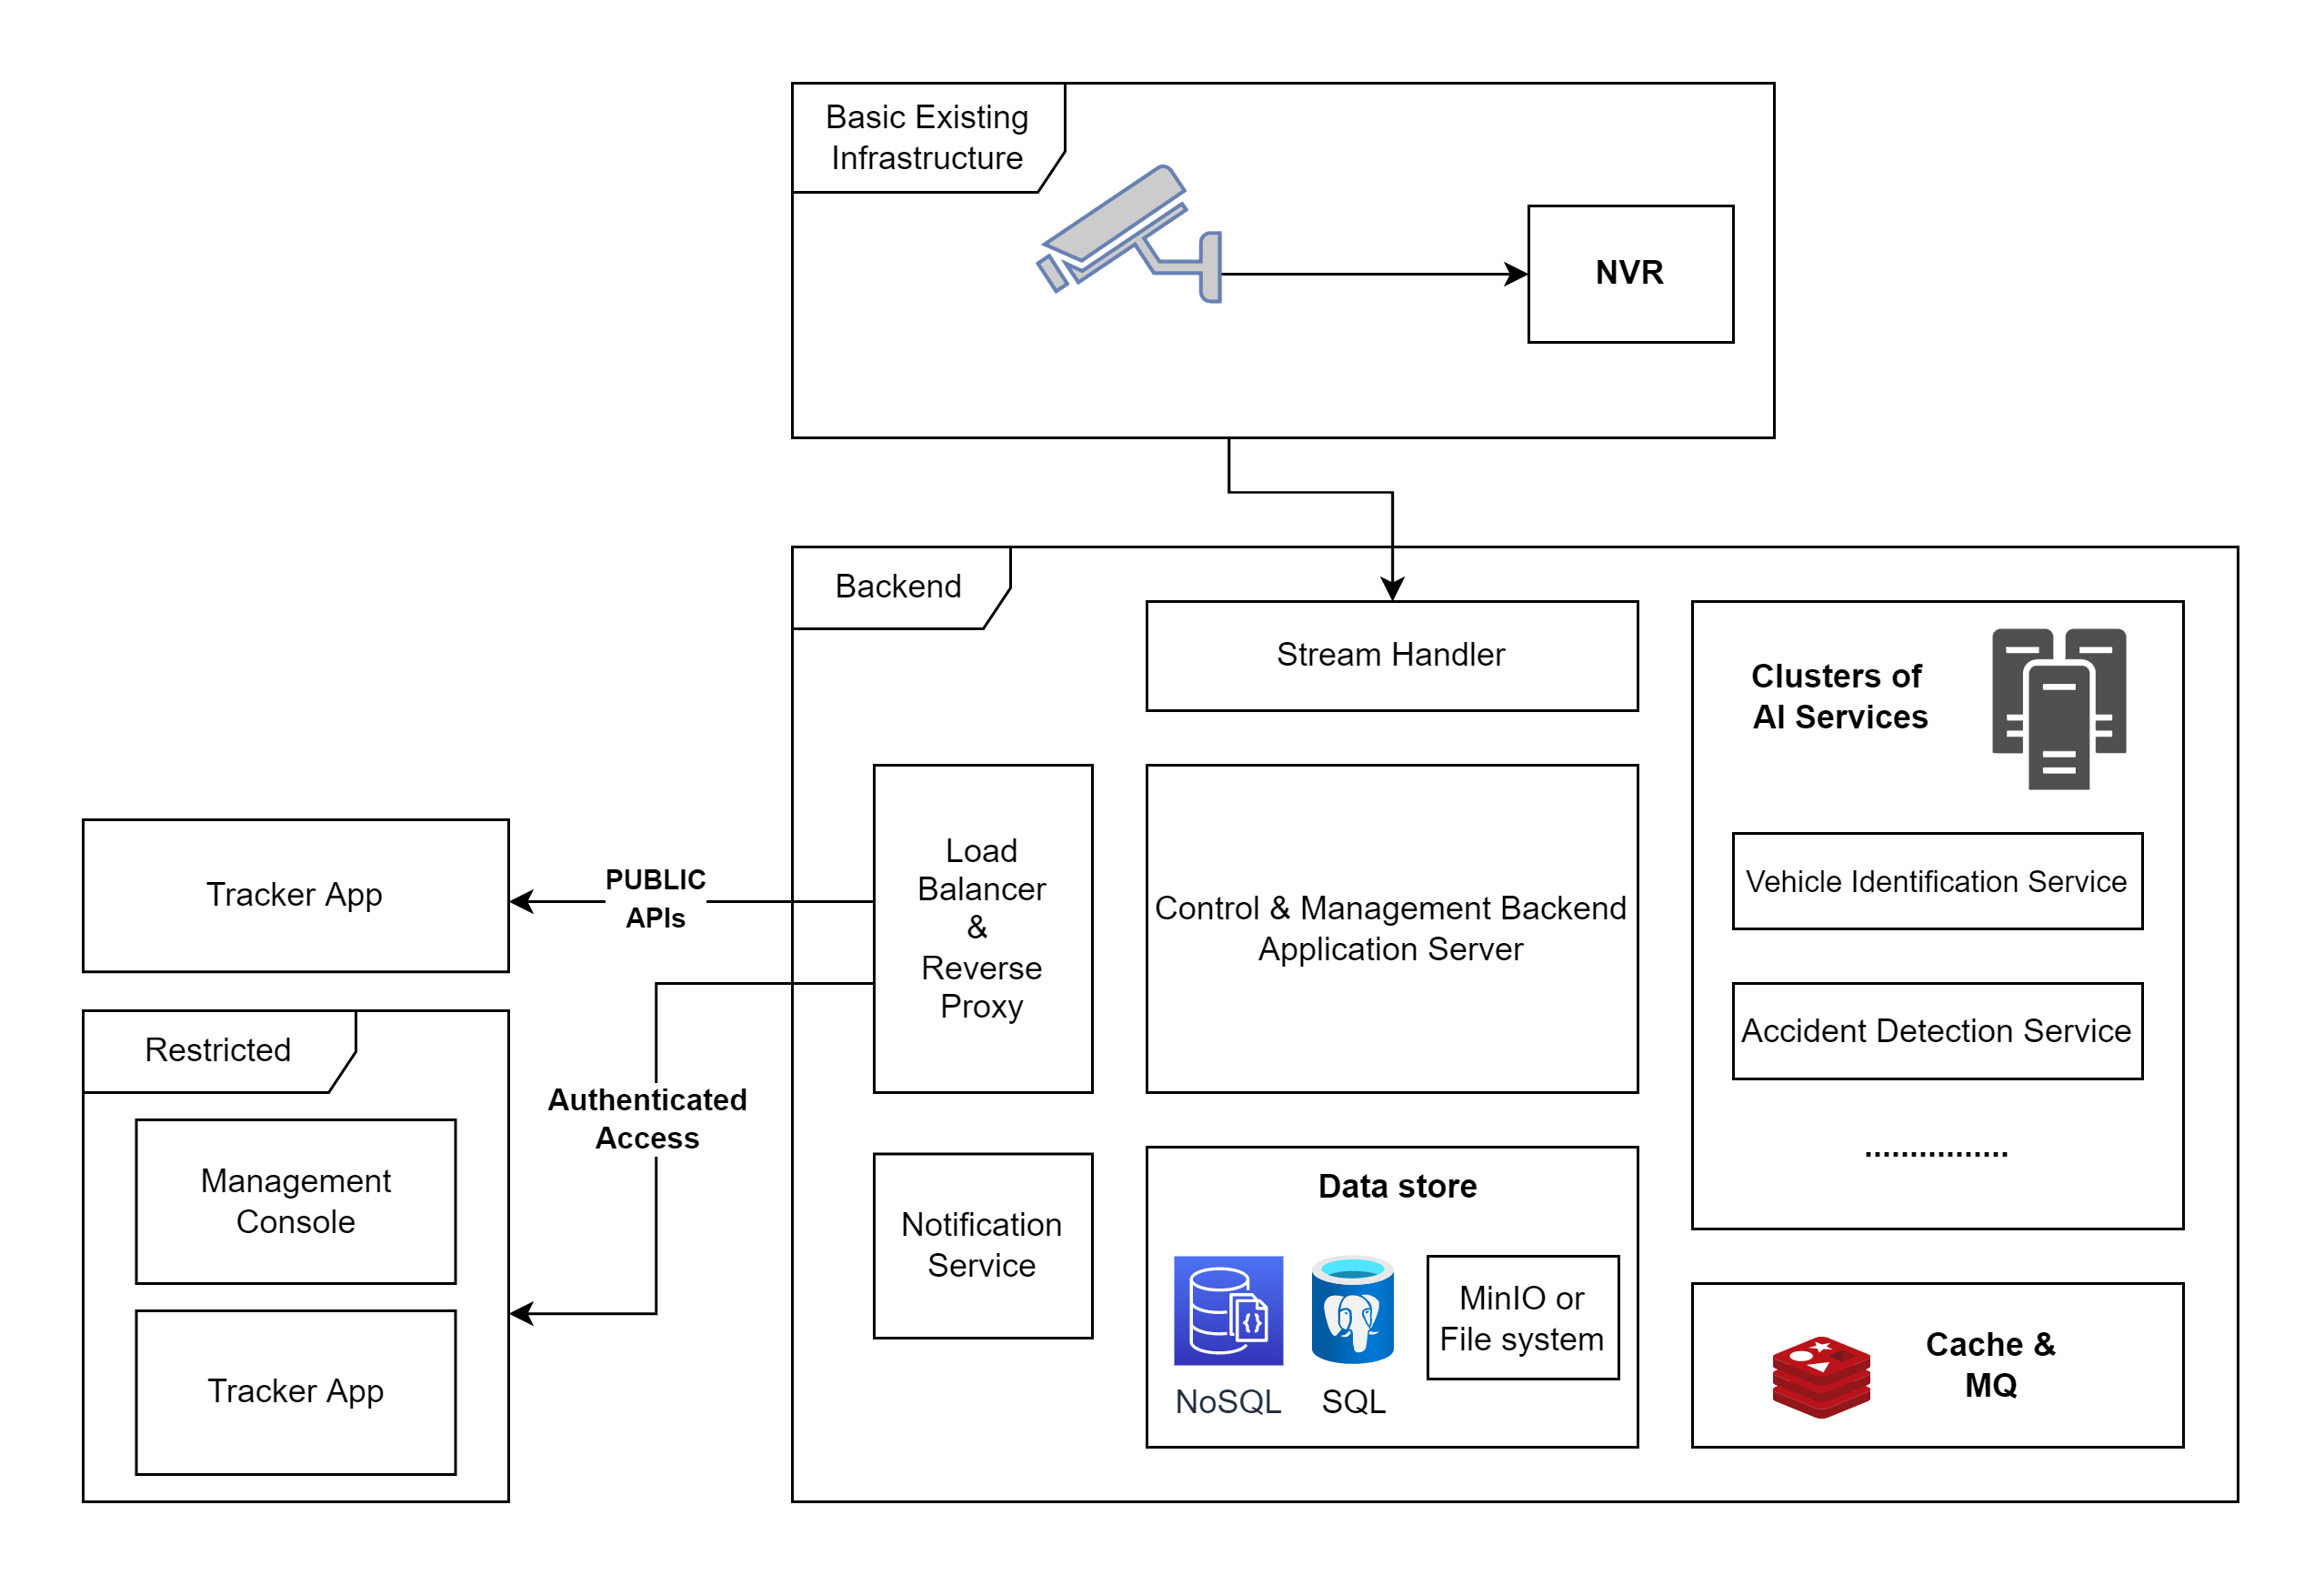
\includegraphics[width=\linewidth]{res/architecture_high_level}
		\end{center}
	\end{frame}

	\begin{frame}{Workflow Pipeline 1}
		\begin{center}
			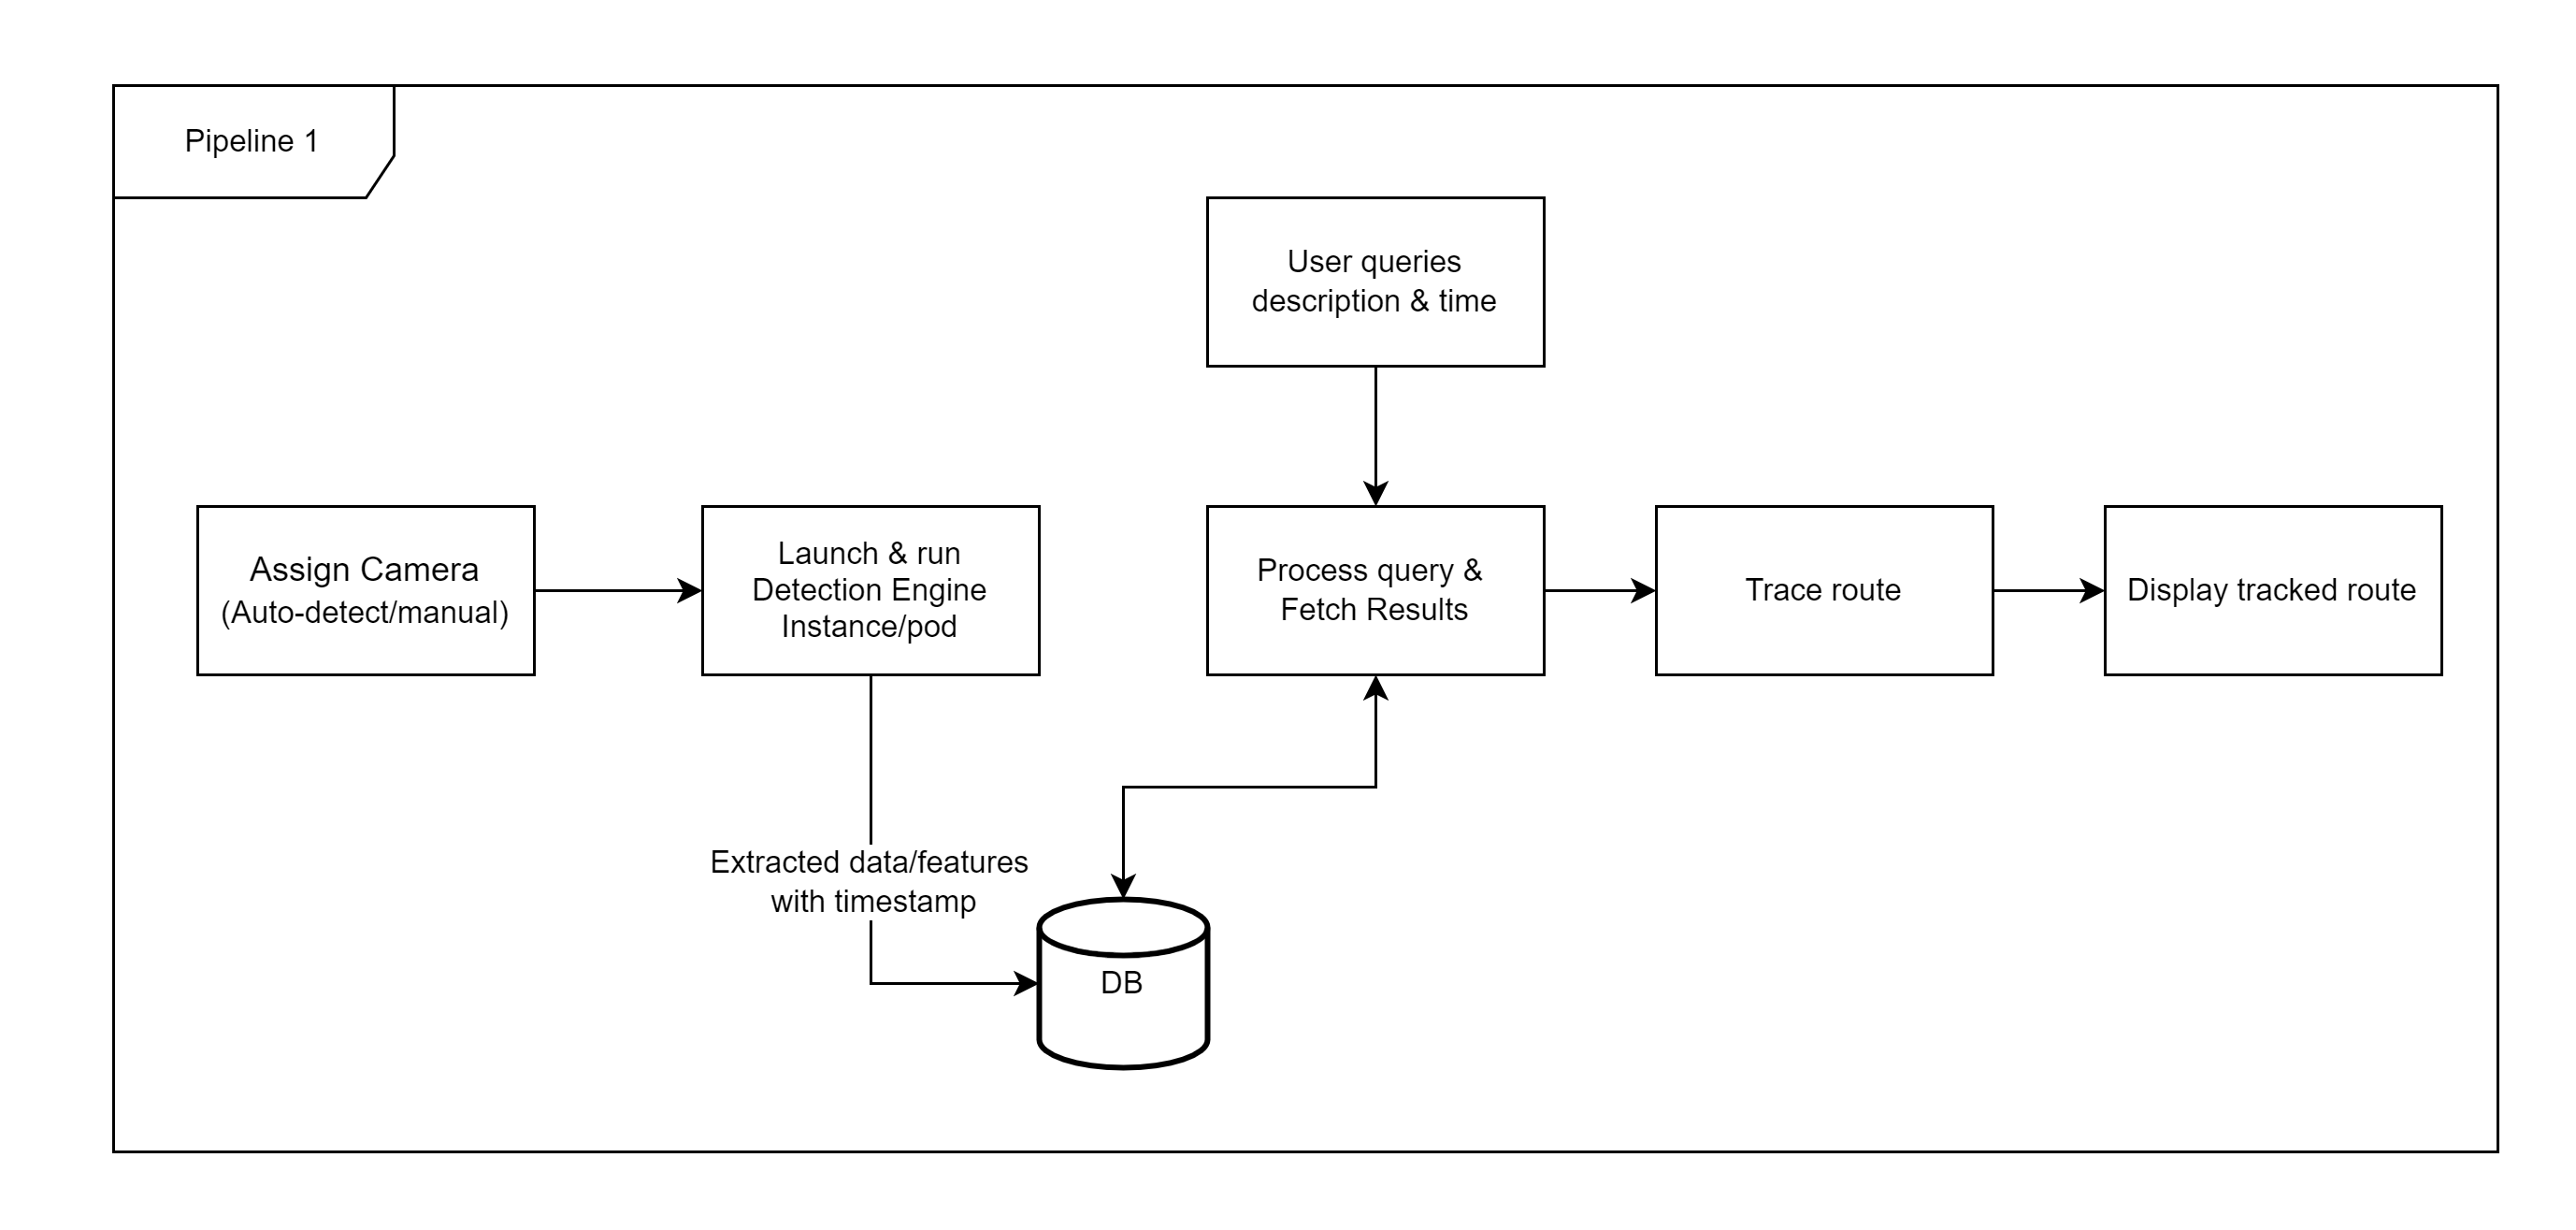
\includegraphics[width=\linewidth]{res/pipeline1}
		\end{center}
	\end{frame}

	\begin{frame}{Workflow Pipeline 2}
		\begin{center}
			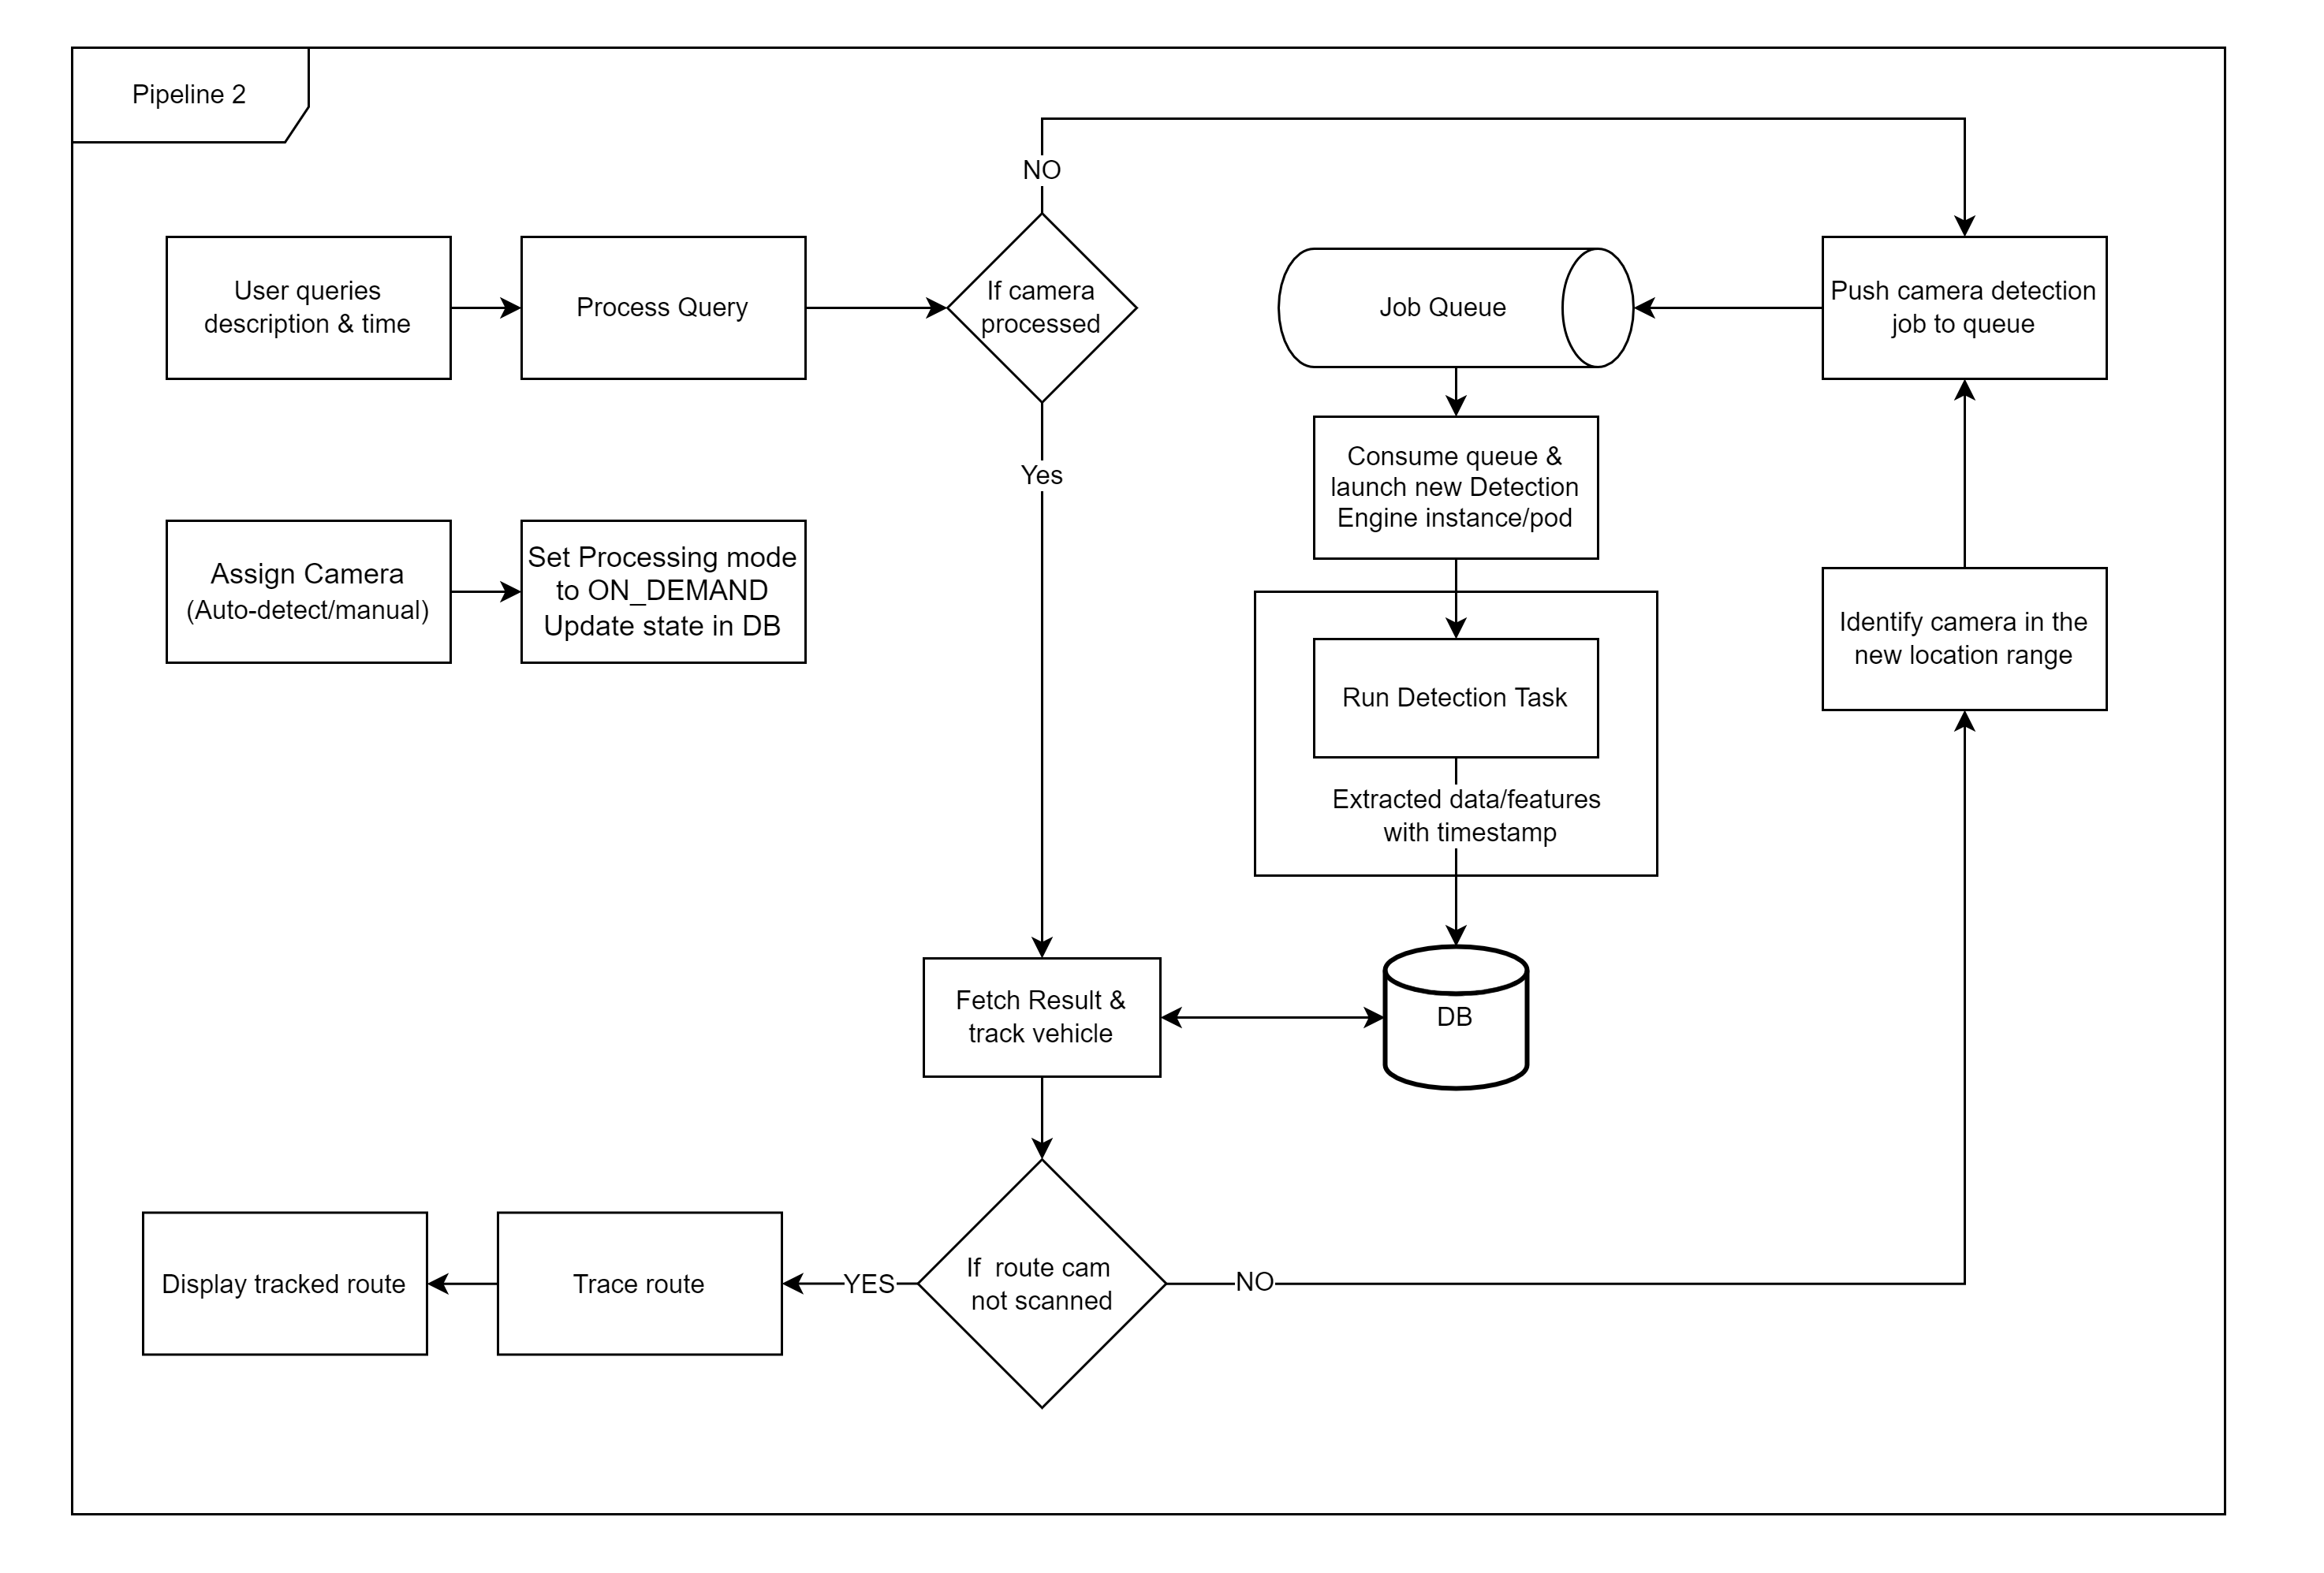
\includegraphics[width=\linewidth]{res/pipeline2}
		\end{center}
	\end{frame}

	\begin{frame}{Camera Feed Live Stream}
		\begin{center}
			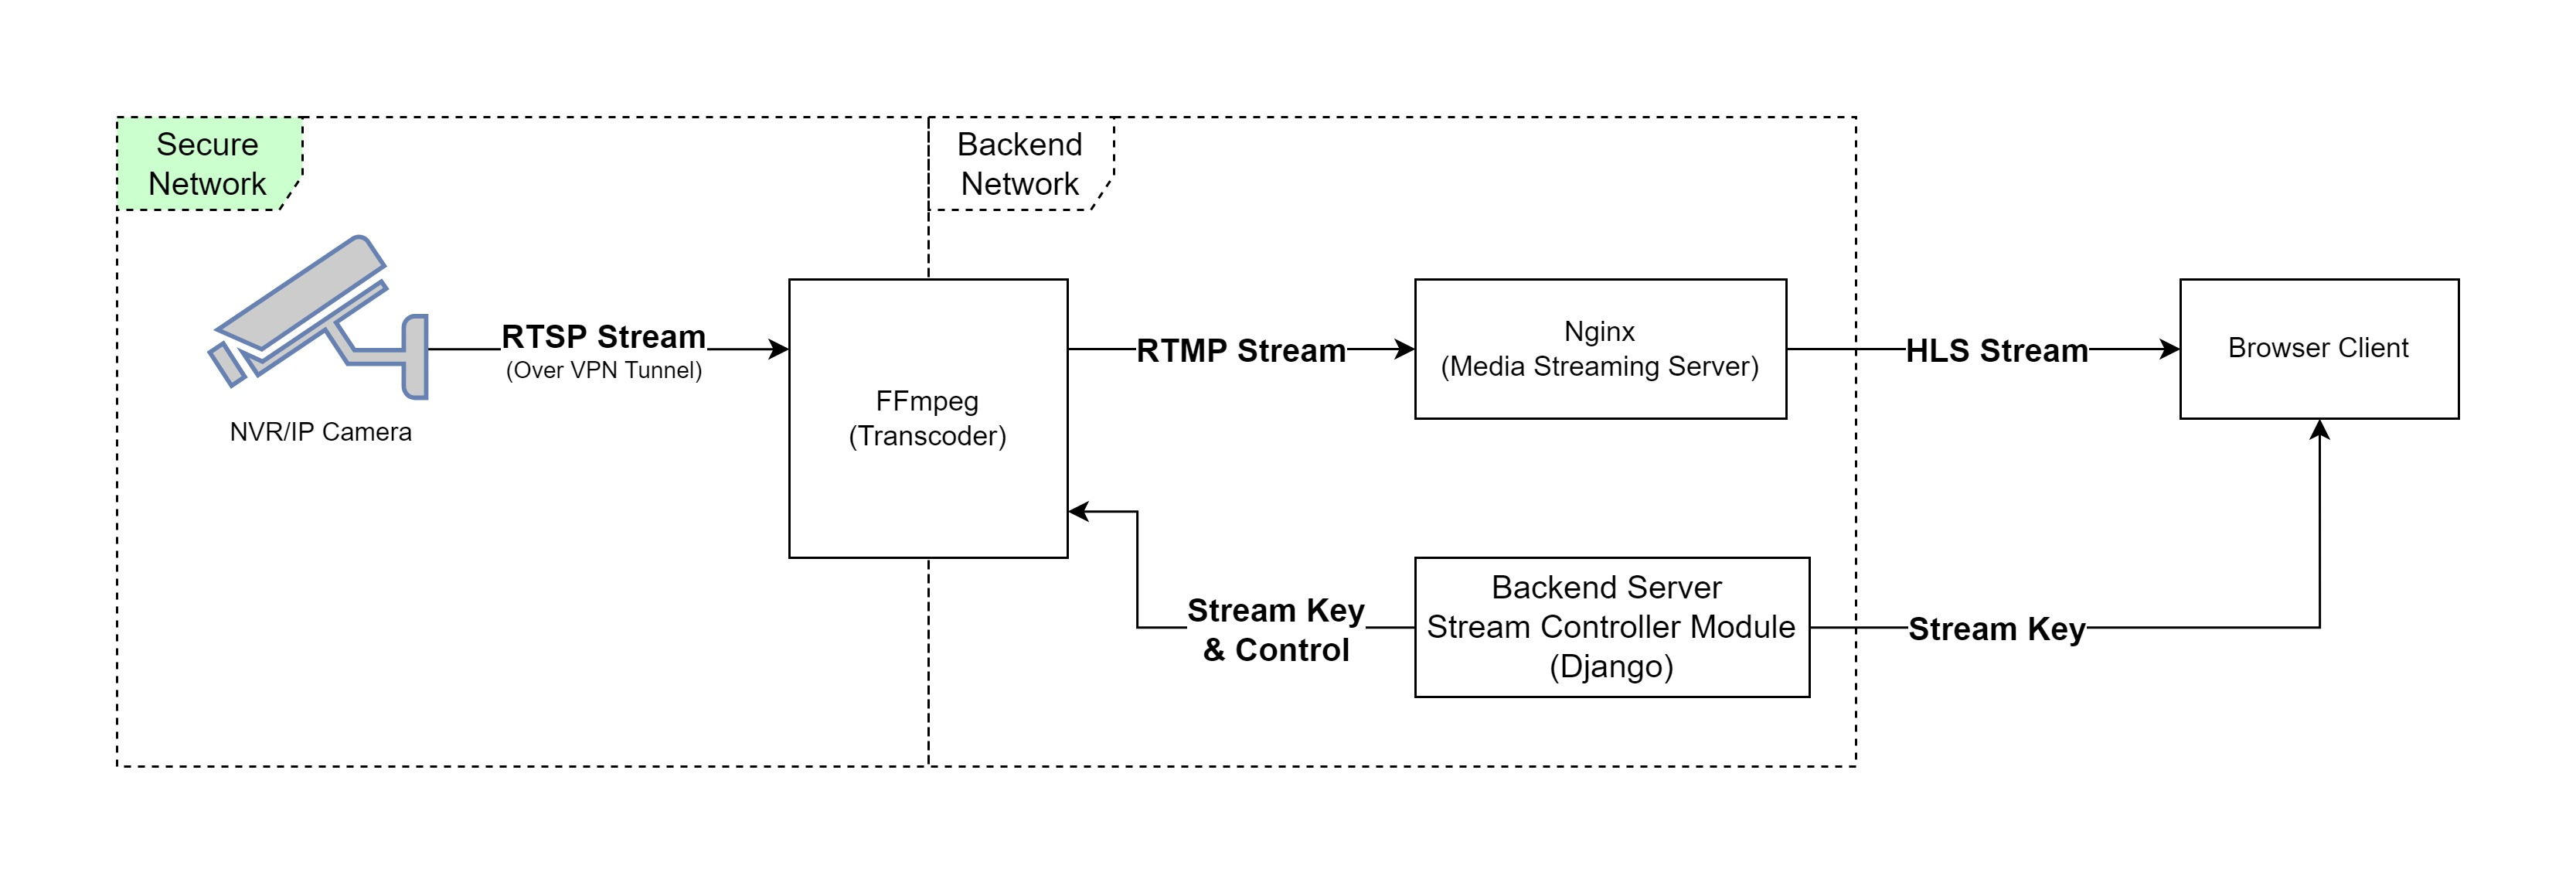
\includegraphics[width=\linewidth]{res/live_stream_arch.jpg}
		\end{center}
	\end{frame}
		
	\subsection{UI Design}
	\begin{frame}{Login Page}
		\begin{center}
			 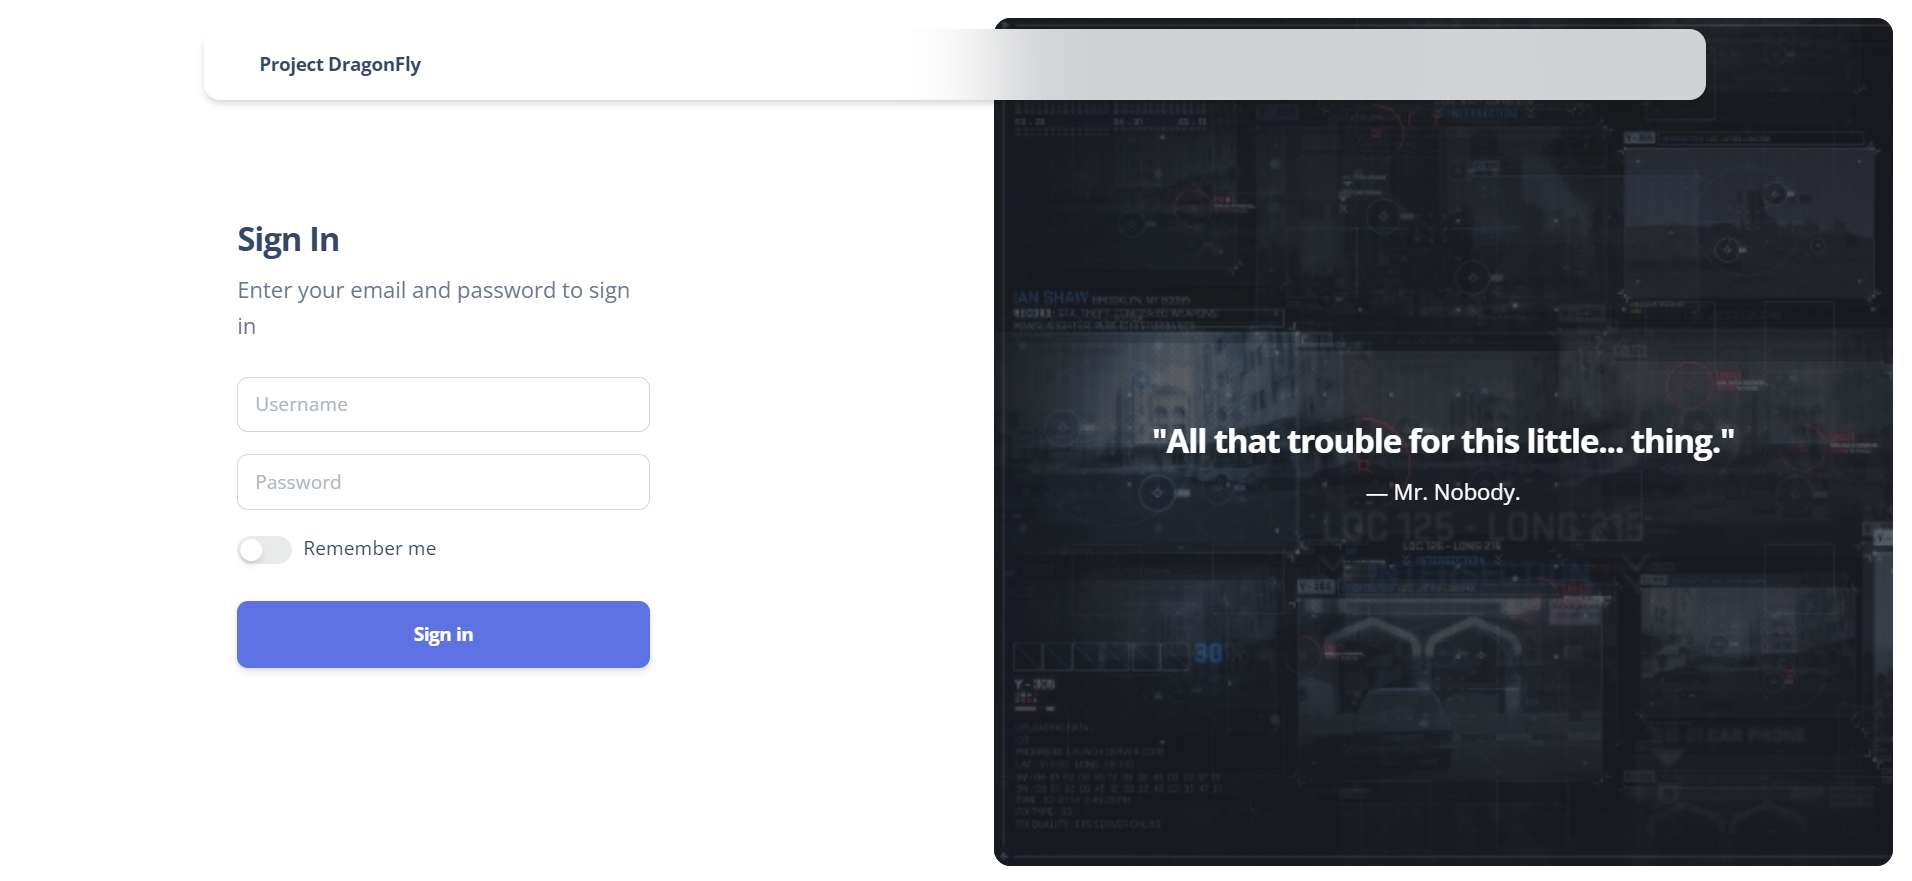
\includegraphics[width=\linewidth]{res/login.png}
		\end{center}
 	\end{frame}
	 
	\begin{frame}{Home Screen}
		\begin{center}
			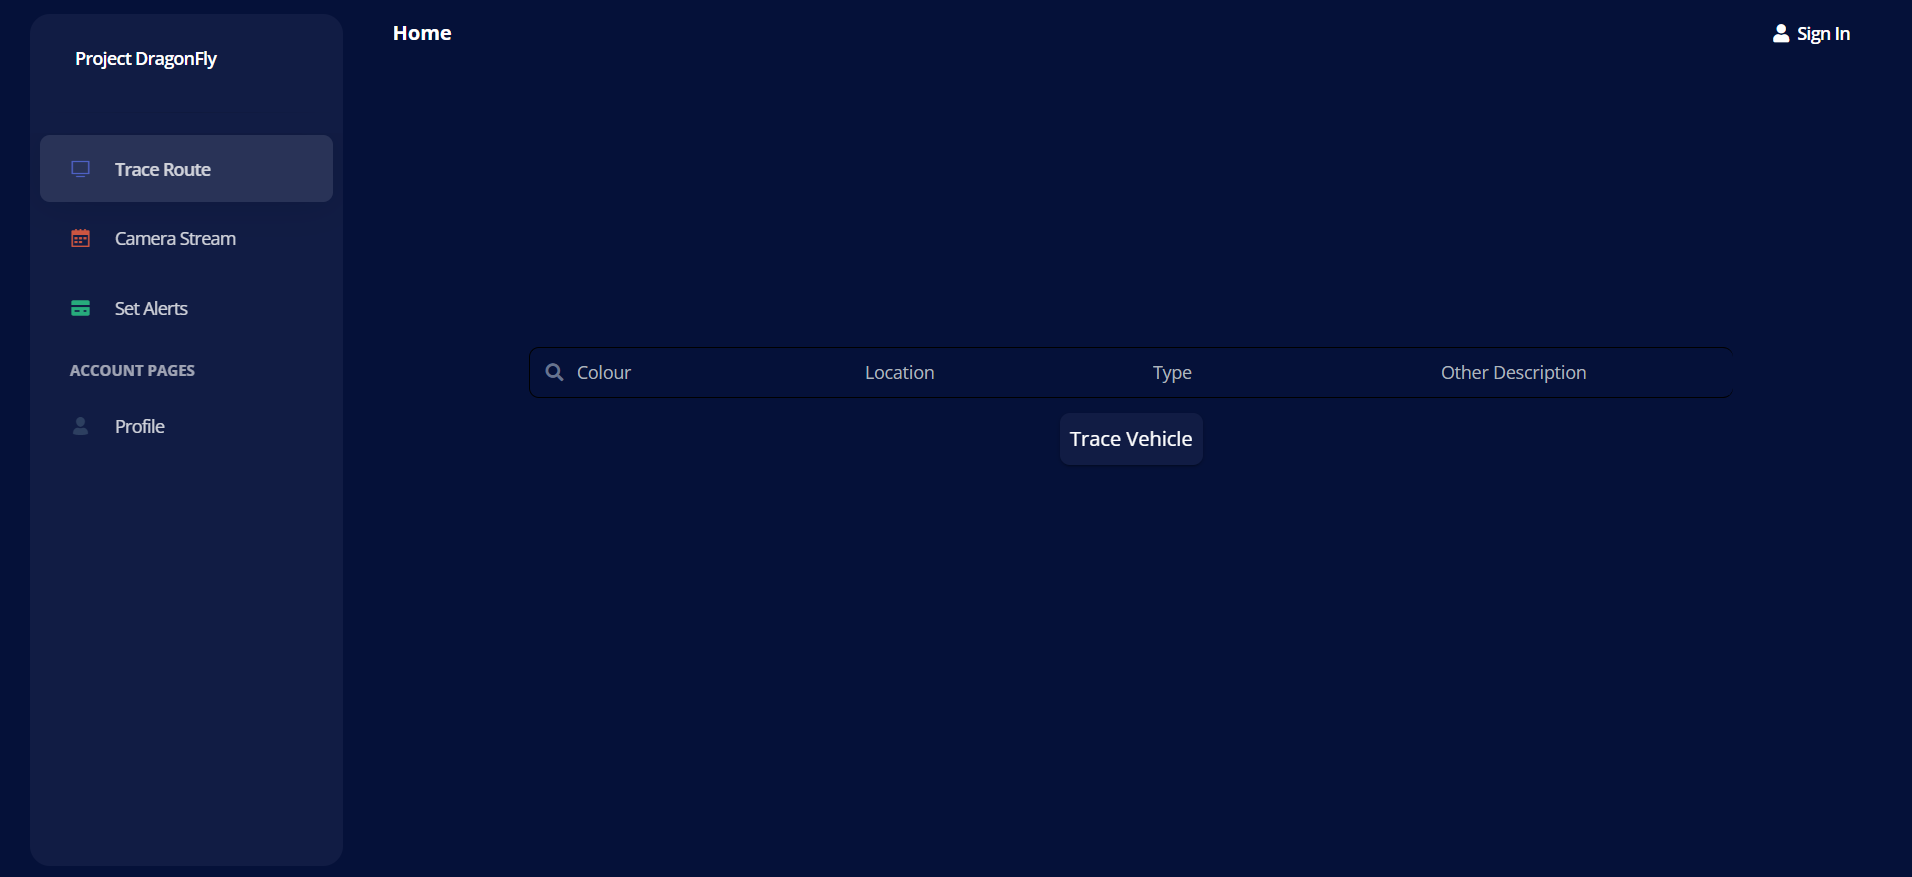
\includegraphics[width=\linewidth]{res/home.png}
		\end{center}
	\end{frame}

 
	 \begin{frame}{Tracking Vehicle}
	 	\begin{center}
	 		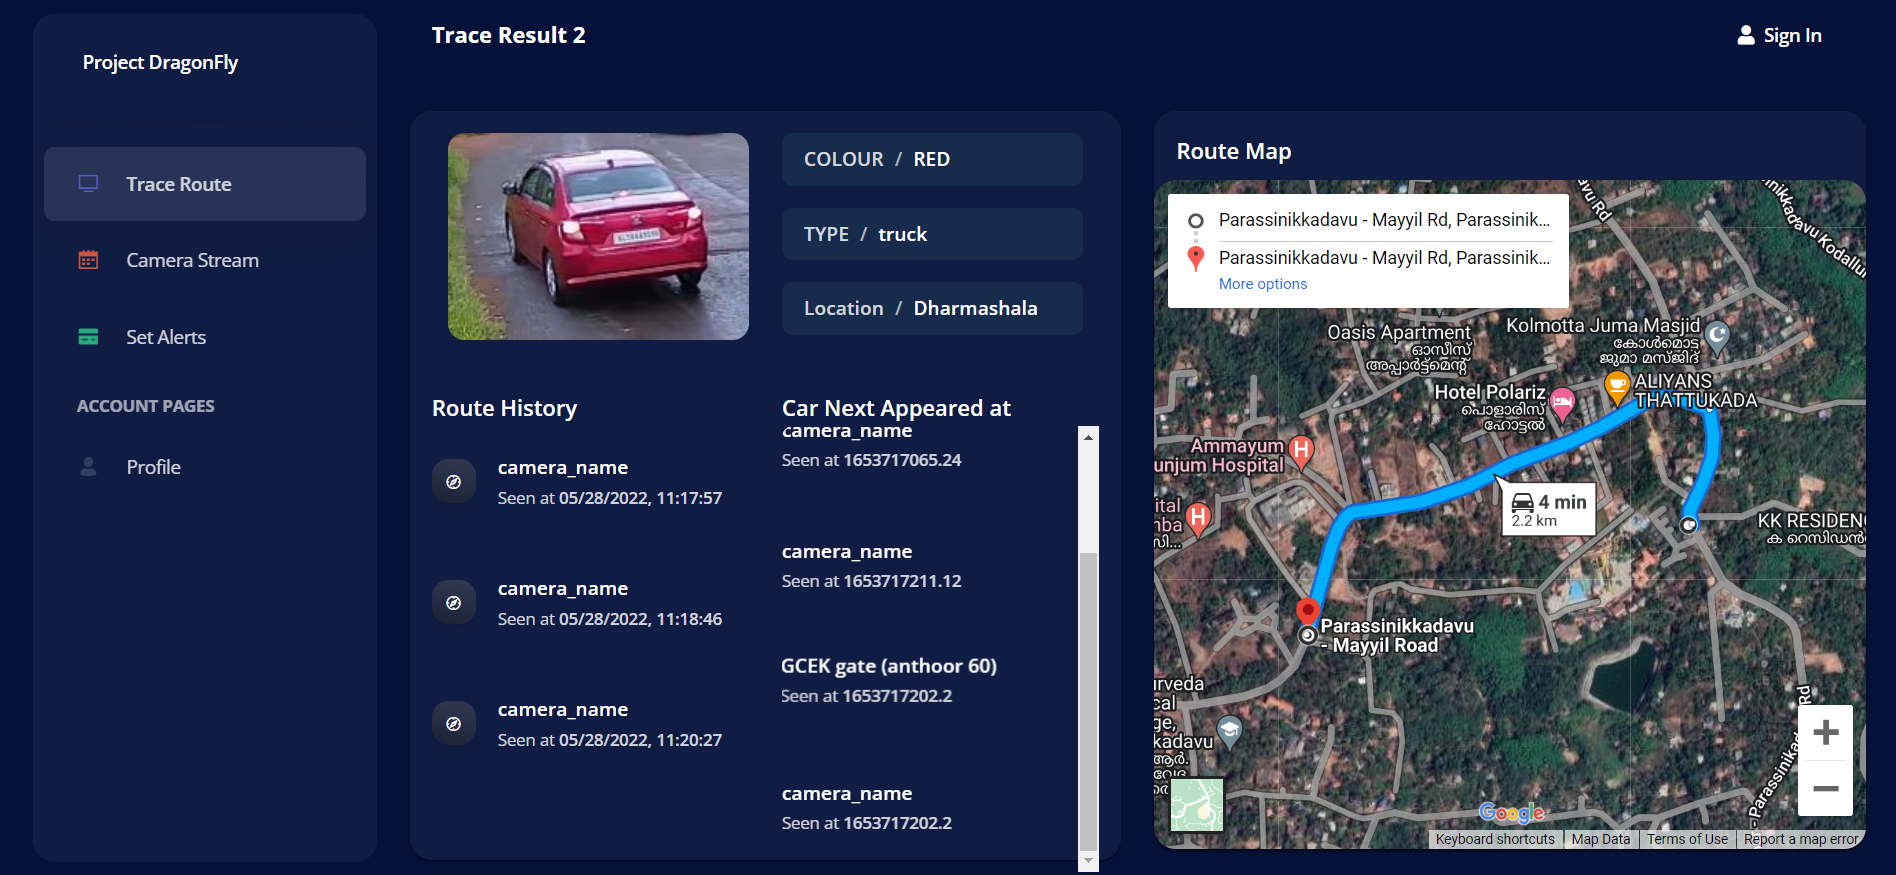
\includegraphics[width=\linewidth]{res/tracing.png}
	 	\end{center}
	 \end{frame}
 
	 \begin{frame}{Building Route Map}
		\begin{center}
			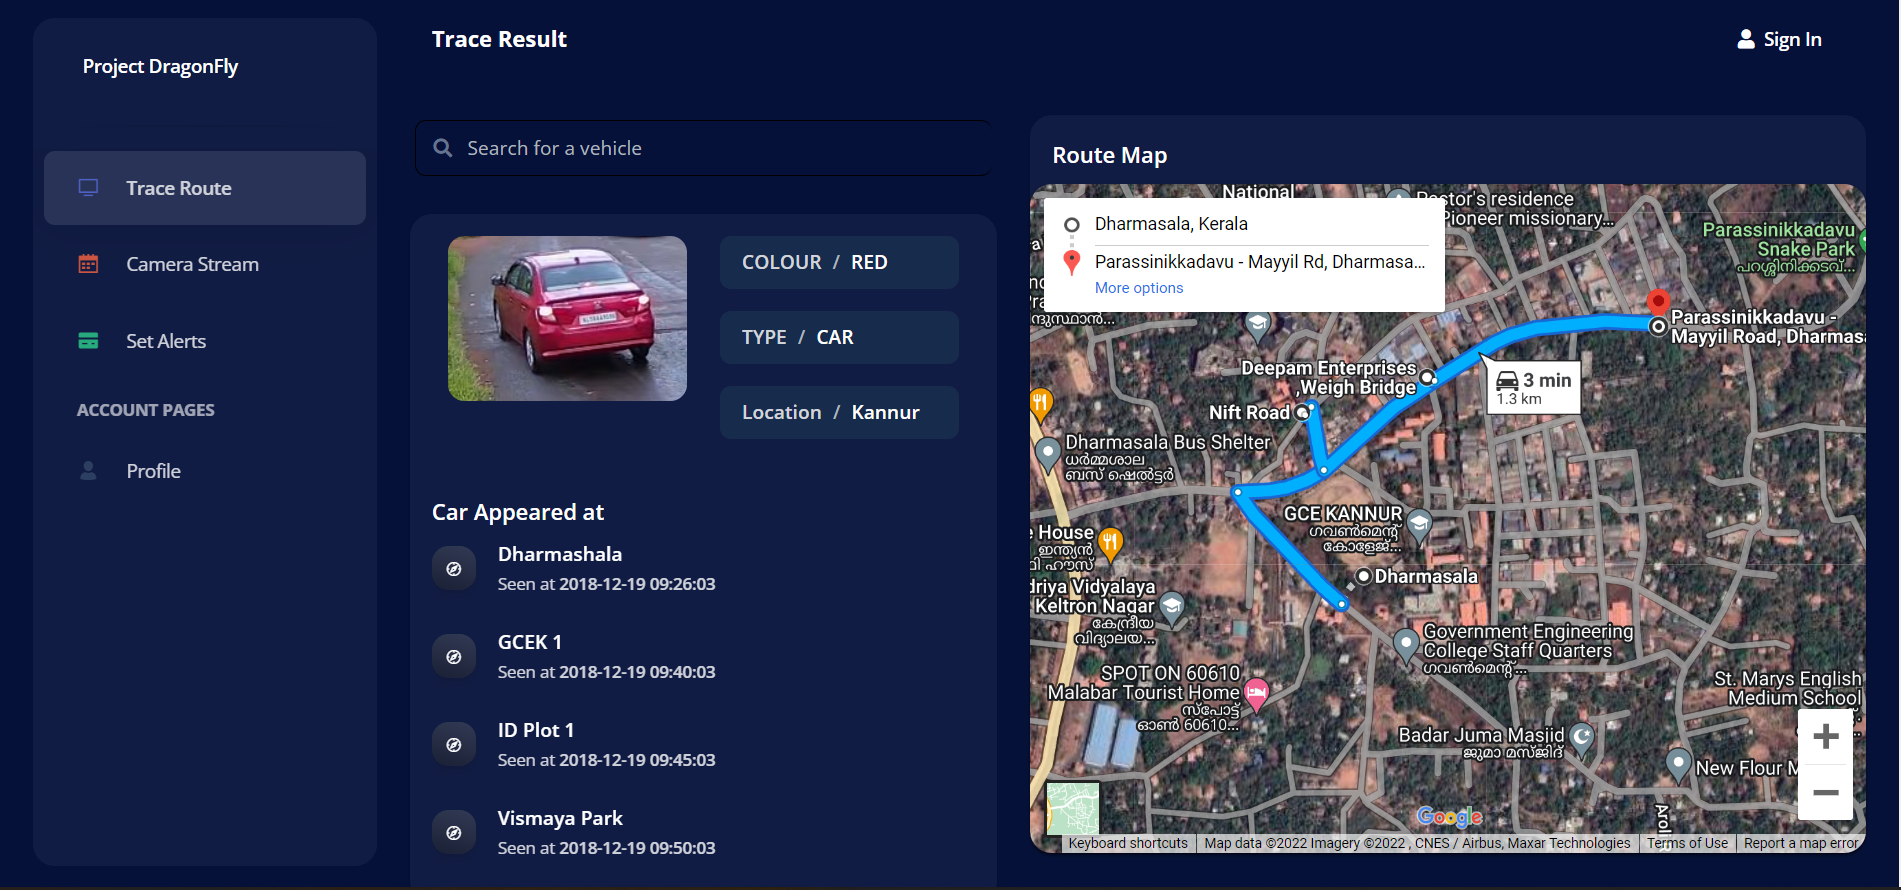
\includegraphics[width=\linewidth]{res/result.png}
		\end{center}
	\end{frame}

	\begin{frame}{Camera Feed Live Streaming}
		\begin{center}
			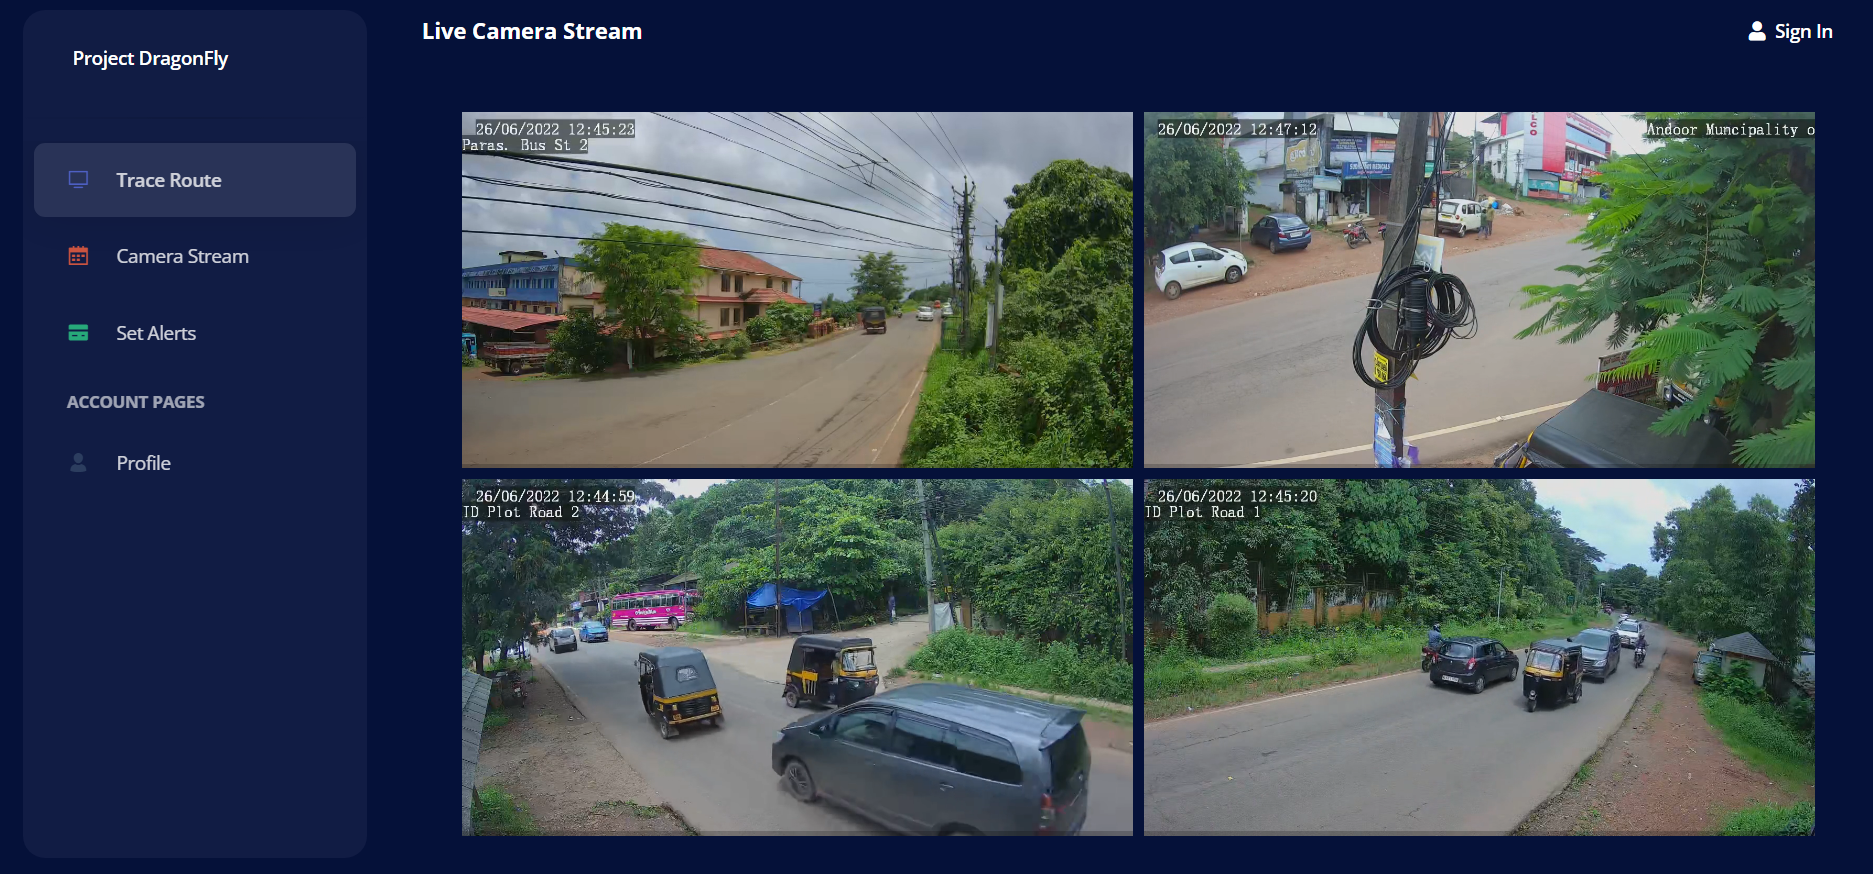
\includegraphics[width=\linewidth]{res/live_stream.png}
		\end{center}
	\end{frame}

	\begin{frame}{Vehicle Image Dictionary Framework}
		\begin{center}
			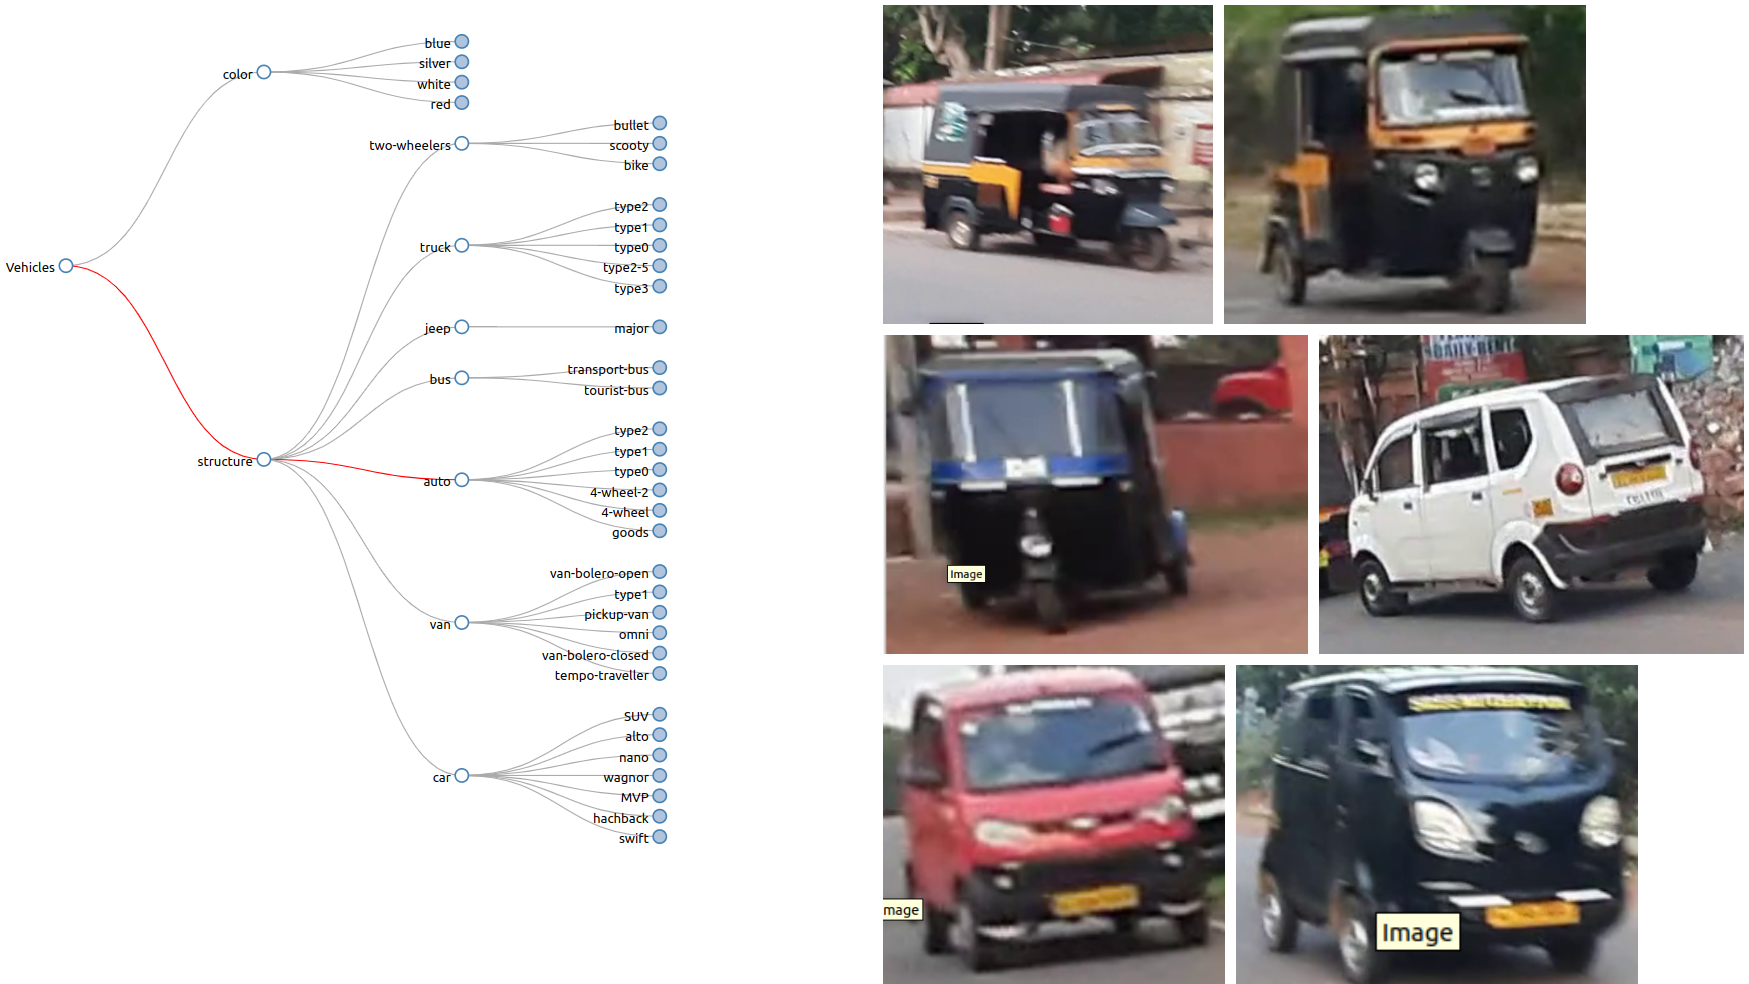
\includegraphics[width=\linewidth]{res/image_dictionary.png}
		\end{center}
	\end{frame}


	\subsection{AI Models}
	\begin{frame}{YOLOv4}
		\framesubtitle{Architecture}
		\begin{center}
			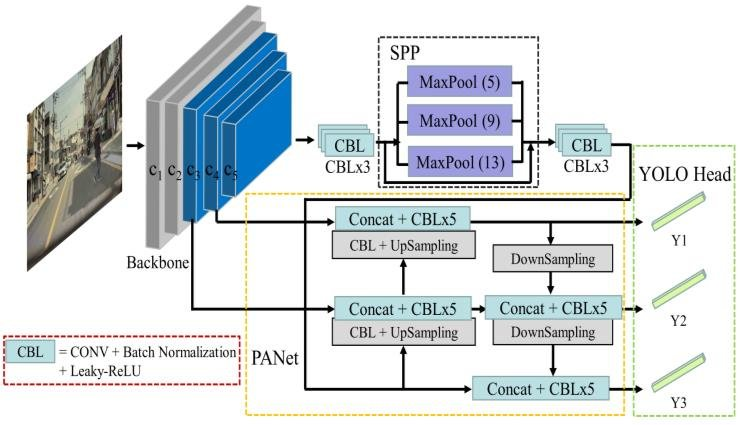
\includegraphics[width=0.8\linewidth]{res/YOLOV4-research-gate.png}
		\end{center}
		Image imported from \link{https://www.researchgate.net/figure/Overall-structure-of-YOLOv4-including-CSPDarknet-backbone-SPPnet-PANet-and-3-YOLO\_fig2\_344919620}{researchgate}. Find the implemented model architecture from \link{https://github.com/Project-Dragon-Fly/Dragon-Fly-Slides/blob/main/final-implementation-review/res/yolov4-vehicle.svg}{here}.
	\end{frame}

	\begin{frame}{YOLOv4}		
		\framesubtitle{Model Parameters}
		\begin{table}[]
			\centering
			\resizebox{\textwidth}{!}{%
				\begin{tabular}{|l|l|}
					\hline
					Input size            & 416 * 416                    \\ \hline
					Input Channels            & 3   \\ \hline
					Batch size             & 32                          \\ \hline
					learning rate    & 0.0013 \\ \hline								Final input to yolo layer        & [256*256],[512*512],[1024*1024]                       \\ \hline
					Total Layers               & 162                     \\ \hline
					
					Target Classes & \begin{tabular}[c]{@{}l@{}}
						auto, bus, tempo traveler, tractor, \\
						truck, van, two wheeler, car, jcb\end{tabular} \\ \hline
				\end{tabular}%
			}
		\end{table}
	\end{frame}

	\begin{frame}{YOLOv4}		
		\framesubtitle{Model Training}
		\begin{table}[]
			\centering
			\resizebox{\textwidth}{!}{%
				\begin{tabular}{|l|l|}
					\hline
					Framework used            & DarkNet                    \\ \hline
					Initial weight            & official 80 class weight   \\ \hline
					Target classes            & 9                          \\ \hline
					Platform for training     & Google Colab + Workstation \\ \hline
					Current mAP               & 97.7 \%                    \\ \hline
					Current Iterations        & 7300                       \\ \hline
					DataSet & \begin{tabular}[c]{@{}l@{}}500 till 2800 iteration\\ 733 till 5300 iteration\\
					1559 afterwards\end{tabular} \\ \hline
					Approx Hrs Spent training & 35-48 hrs                \\ \hline
				\end{tabular}%
			}
		\end{table}
	\end{frame}

	\begin{frame}[allowframebreaks]{Dataset - Kaggle}
		Fetched from \link{https://www.kaggle.com/datasets/dataclusterlabs/indian-vehicle-dataset}{Kaggle}. Used labelImg to label images. 
		\begin{table}[]
			\centering
			\begin{tabular}{|l|l|}
				\hline
				\textbf{Label Name}   & \textbf{Frequency}    \\ \hline
				two wheeler           & 557                   \\ \hline
				truck                 & 354                   \\ \hline
				auto                  & 297                   \\ \hline
				car                   & 233                   \\ \hline
				bus                   & 220                   \\ \hline
				tractor               &  133                  \\ \hline
				van                   & 101                   \\ \hline
				jcb                   & 1                     \\ \hline
				\textbf{Total Boxes}  & \textbf{1956}       \\ \hline
				\textbf{Total Images} & \textbf{733}        \\ \hline
			\end{tabular}
		\end{table}
		
		
		
		\newpage
		\begin{figure}
			\includegraphics[width=0.24\linewidth]{"res/data_set1/image1"} \hfill
			\includegraphics[width=0.24\linewidth]{"res/data_set1/image2"} \hfill
			\includegraphics[width=0.24\linewidth]{"res/data_set1/image3"} \hfill
			\includegraphics[width=0.24\linewidth]{"res/data_set1/image4"}
		\end{figure}
	\end{frame}
	
	
	\begin{frame}[allowframebreaks]{Dataset - Camera Network}
		Fetched from camera infrastructure. Used labelImg to label images.
		\begin{center}
			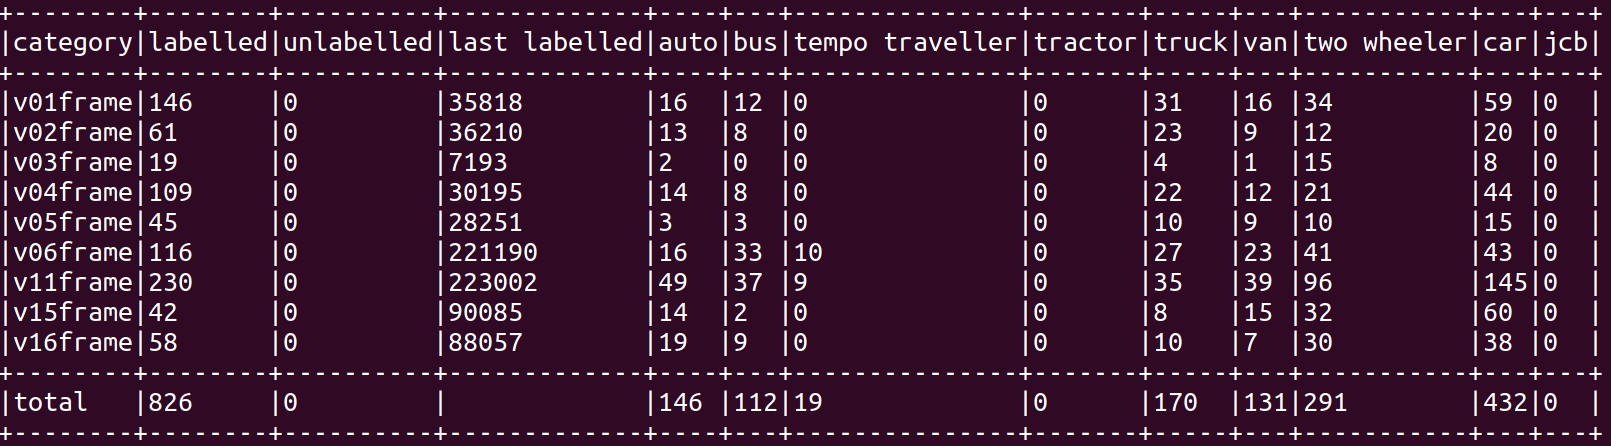
\includegraphics[width=\linewidth]{res/data_set2/custom_label_stat}
		\end{center}
		
		\newpage
		\begin{figure}
			\includegraphics[width=0.48\linewidth]{"res/data_set2/image1"} \hfill
			\includegraphics[width=0.48\linewidth]{"res/data_set2/image2"}
			\\[\smallskipamount]
			\includegraphics[width=0.48\linewidth]{"res/data_set2/image3"} \hfill
			\includegraphics[width=0.48\linewidth]{"res/data_set2/image4"}
		\end{figure}
	\end{frame}


	\begin{frame}{deepSORT}
		\begin{center}
			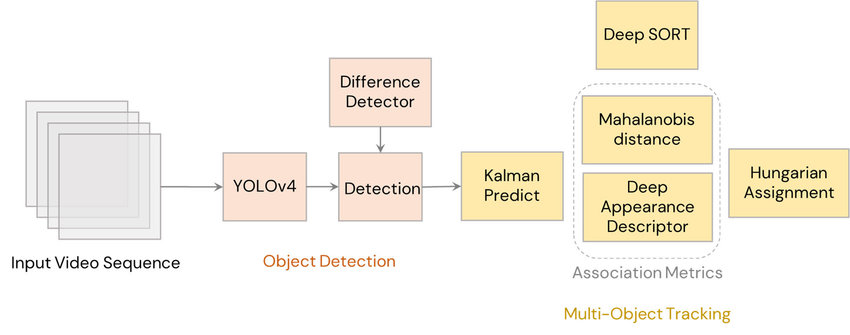
\includegraphics[width=0.95\linewidth]{res/deepSORT.png}
		\end{center}
		Image imported from \link{https://www.researchgate.net/figure/Architecture-of-Deep-SORT-Simple-online-and-real-time-tracking-with-deep-association\_fig2\_353256407}{researchgate}.
	\end{frame}

	\begin{frame}{Siamese Network}
		\begin{center}
			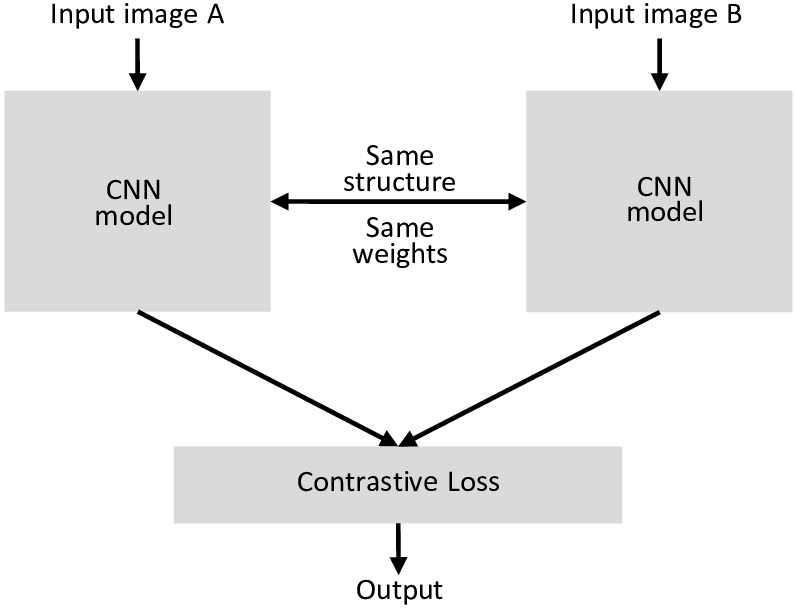
\includegraphics[height=0.6\textheight]{res/siamese-network.png}
		\end{center}
		Image imported from \link{https://www.researchgate.net/figure/Structure-of-the-Siamese-network\_fig1\_327494280}{researchgate}.
	\end{frame}

	\begin{frame}{Algorithm}
		\framesubtitle{Integrate algorithms}
		\begin{center}
			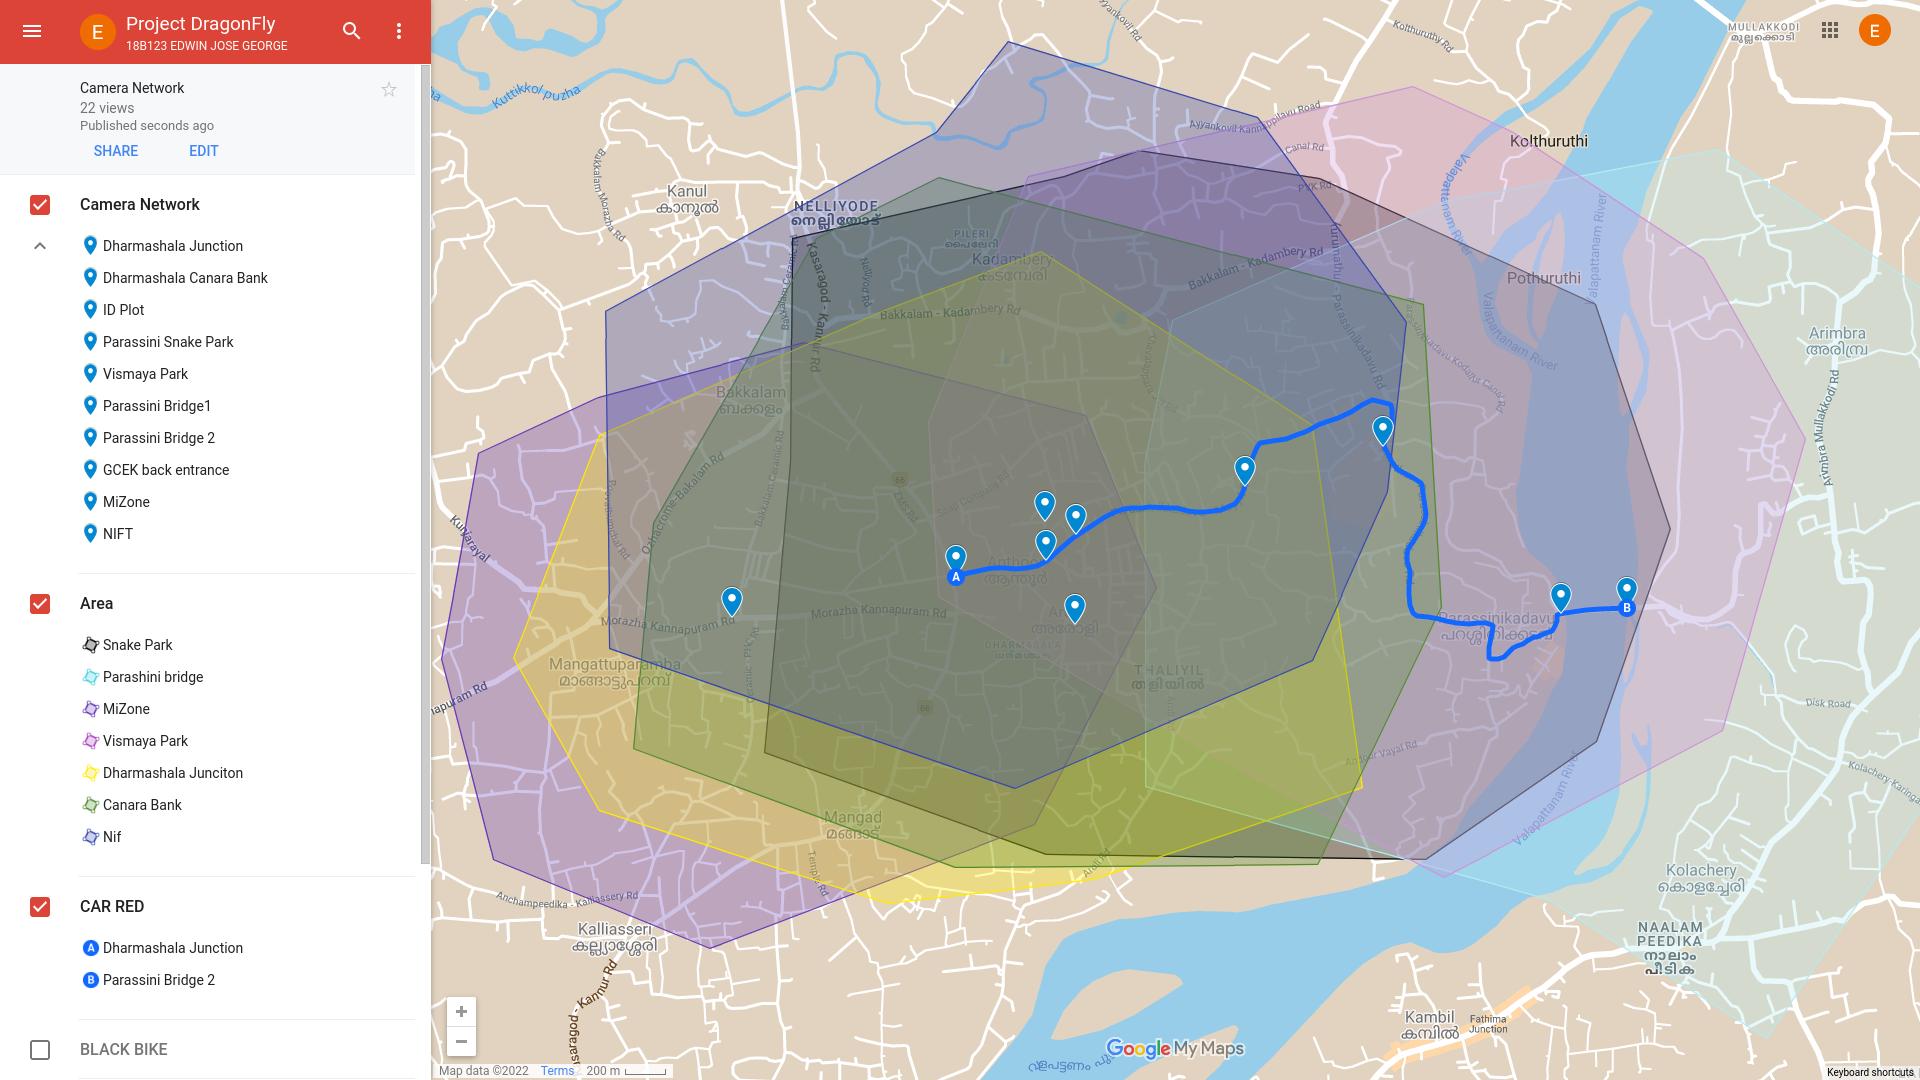
\includegraphics[height=0.7\textheight]{res/camera_network_demo.png}
		\end{center}
		Created with \link{https://www.google.com/maps/d/edit?mid=1s2ST5x4nn-EK3JqU-c9EEGASRq5Ini0&usp=sharing}{Google Maps}
	\end{frame}
	
	


	%---------------------------------------------------------------------------
	% RESULTS ------------------------------------------------------------------
	%---------------------------------------------------------------------------

	\section{Results}
	\subsection{AI model}
	\begin{frame}{YOLOv4 model}
		\framesubtitle{Training - Loss and Accuracy chart}
		\begin{center}
			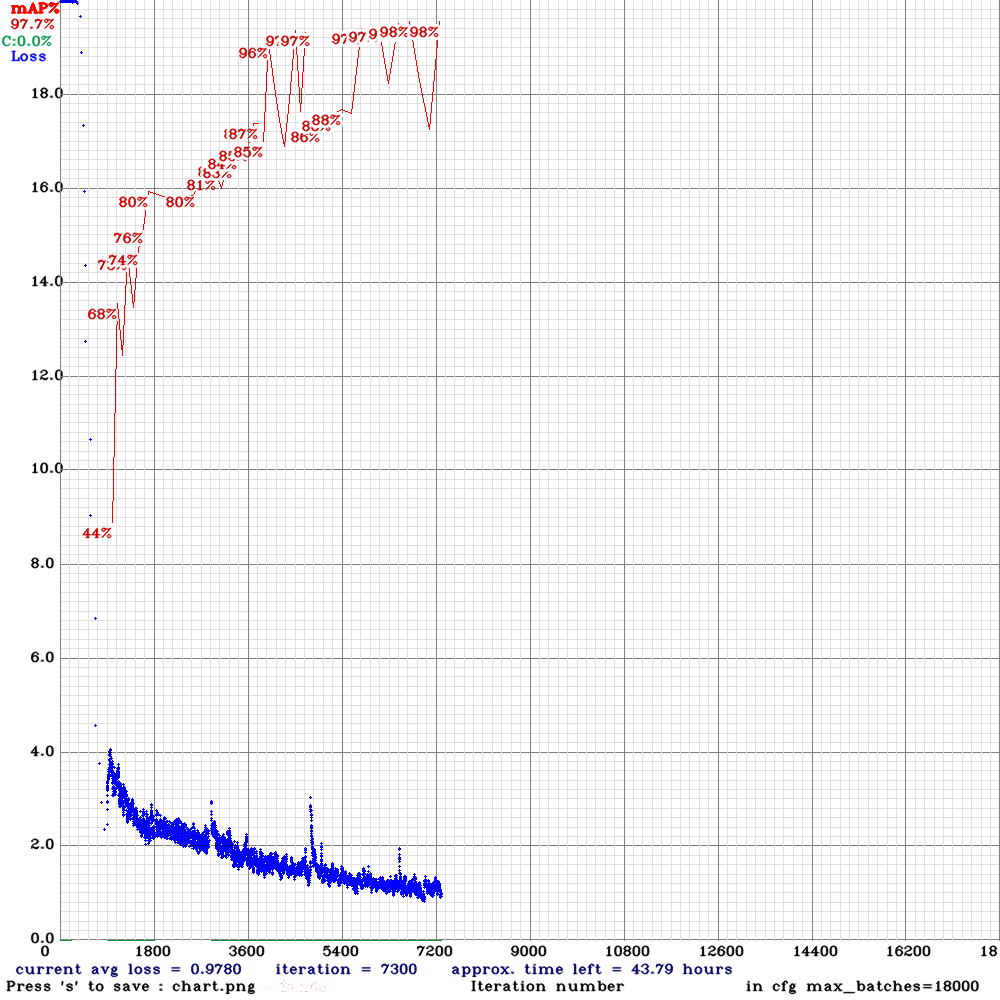
\includegraphics[height=0.7\textheight]{res/darknet_training_chart}
		\end{center}
	\end{frame}

	\begin{frame}[allowframebreaks]{YOLOv4 model Accurancy}
		\framesubtitle{Matrix}
		\begin{table}[]
			\begin{tabular}{|l|l|l|l|}
				\hline
				Class label    & True Positive & False Positive & Avg Precision \\ \hline
				auto           & 424           & 38             & 98.25\%       \\ \hline
				bus            & 327           & 42             & 99.57\%       \\ \hline
				tempo traveler & 76            & 7              & 97.12\%       \\ \hline
				tractor        & 130           & 2              & 98.44\%       \\ \hline
				truck          & 516           & 33             & 99.28\%       \\ \hline
				van            & 227           & 22             & 98.14\%       \\ \hline
				two wheeler    & 770           & 241            & 91.62\%       \\ \hline
				car            & 644           & 91             & 96.99\%       \\ \hline
				jcb            & 0             & 0              & 100.00\%      \\ \hline
			\end{tabular}
		\end{table}
		Detections count = 12349 \\
		Unique truth count = 3257
		\newpage
		
		\begin{table}[]
			\begin{tabular}{|l|l|}
				\hline
				Precision          & 87\%    \\ \hline
				Recall             & 96\%    \\ \hline
				F1-score           & 91\%    \\ \hline
				True Positive      & 3114    \\ \hline
				False Positive     & 476     \\ \hline
				False Negative     & 134     \\ \hline
				Avg IoU            & 72.13\% \\ \hline
				Mean Avg precision & 97.71\% \\ \hline
			\end{tabular}
		\end{table}
		Total Detection Time: 1166 Seconds
	\end{frame}

	\begin{frame}{YOLOv4 model}
		\framesubtitle{Prediction}
		\begin{center}
			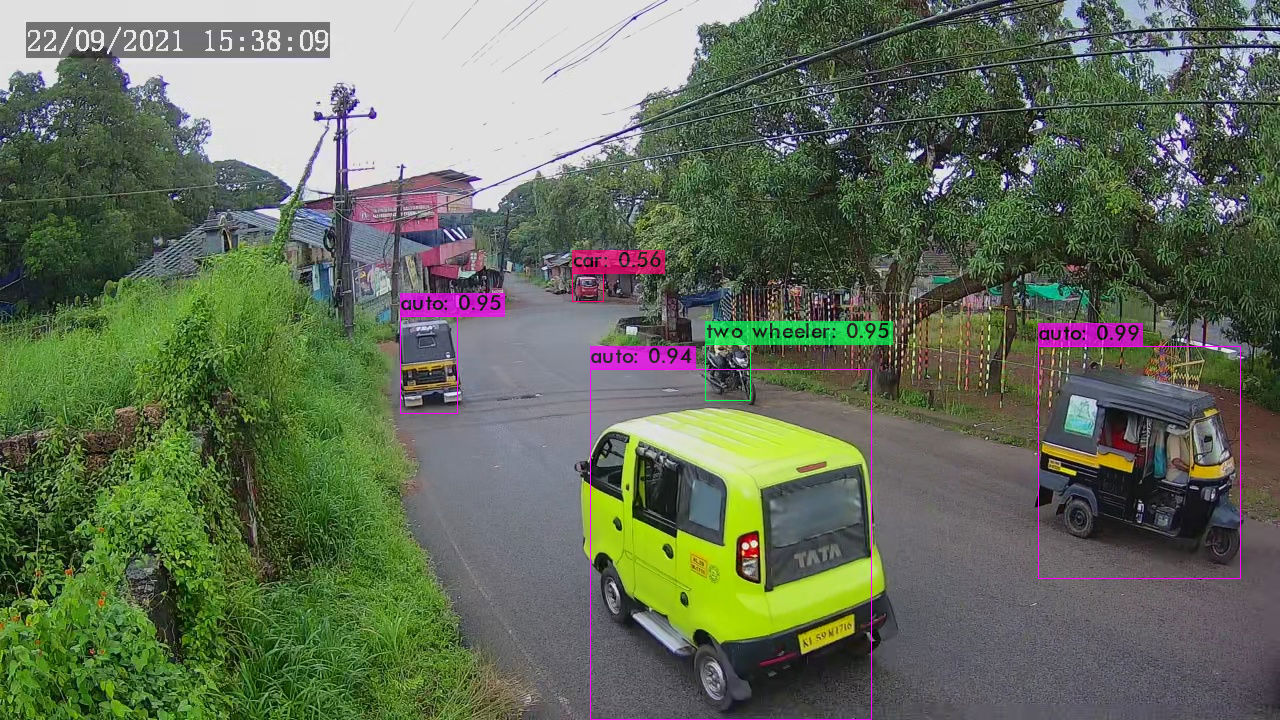
\includegraphics[width=\linewidth]{res/data_set1/predictions}
		\end{center}
	\end{frame}


	\section{Conclusion}
	\begin{frame}{Conclusion}
		\begin{itemize}
			\item The project works over the existing CCTV infrastructure
			\item Detections are retrieved based on user query in web GUI
			\item AI Detection Engine processes camera stream, computing vehicle features
			\item YOLOv4 model computes the bounding box and class confidence
			\item DeepSORT conduct multi-tracking in multiple objects
			\item User can select between alternative detections to generate routemap
			\item Vehicle Routemap is display using Map
			\item User can view live stream of multiple CCTV camera within the app
		\end{itemize}
	\end{frame}
	\begin{frame}[allowframebreaks]{Future Scope}
		\begin{itemize}
			\item Addition of advanced camera and integration of license plate detection, to recognise forged license plate
			\item Training in all weather conditions and higher number of sub-categories
			\item Complete implementation of Siamese Network. 
			\item Search Engines like elastic search and language models for natural interaction and extraction of feature description
			\item Securing IP stream of camera feed using DRM protection.
			\item Using Enteprise Media Servers like Kurento Media Server, Ant Media Server to enable ultra low latency stream relay
			\item Usage of Nvidia MPS and Multi-GPU instances
			\item Use of PP-YOLO with PaddlePaddle framework can boost the overall performance of thedistributed system.
		\end{itemize}
	\end{frame}
\section{References}
\begin{frame}[allowframebreaks]{References}
	\nocite{*}
	\bibliographystyle{IEEEtran}
	\bibliography{IEEEabrv,reference.bib}
\end{frame}

\end{document} 